\documentclass[fleqn,10pt]{wlscirep-authoryear}
\usepackage[utf8]{inputenc}
\usepackage{graphicx}
\usepackage{comment}
\usepackage{subcaption}
\usepackage[T1]{fontenc}
\usepackage{tikz}
\usetikzlibrary{arrows.meta, positioning, shapes.geometric, fit}
\usepackage[most]{tcolorbox}
\usepackage{xcolor}
\usepackage{listings}
\usepackage{tabularx}
\usepackage{booktabs,enumitem,amsmath,amssymb,longtable}
\lstdefinestyle{promptstyle}{backgroundcolor=\color{pastelblue}, basicstyle=\ttfamily\small, breaklines=true, frame=single}

\newtcolorbox{promptbox}[1][]{
  enhanced,
  breakable,
  colback=blue!2!white,
  colframe=black!35,
  boxrule=0.4pt,
  arc=2mm,
  left=1.5mm,
  right=1.5mm,
  top=1mm,
  bottom=1mm,
  opacityback=0.45,
  title=#1,
  fonttitle=\bfseries,
}
\definecolor{pastelblue}{RGB}{220,235,250}
\definecolor{pastelgreen}{RGB}{222,242,222}
\definecolor{pastelyellow}{RGB}{255,248,220}
\definecolor{pastelpurple}{RGB}{235,228,250}

\title{Prompt Composition and Length Trade-offs in Structured Information
Extraction with Large Language Models}
%Hydrological observations from Arctic river sites in the Anadyr–Kolyma basin}



\author[1]{Vadim Tynchenko}
%\author[1]{Dmitry Martysyuk}
\author[1]{Vladimir Nelyub}
\author[1]{Aleksei Borodulin}
%\author[1]{Andrei Gantimurov}
\author[1*]{Ivan Malashin}

%\author[1]{Vadim S. Tynchenko}
%\author[1]{Aleksei S. Borodulin}
%\author[1]{Vladimir A. Neluyb}
%\affil[1]{Affiliation, department, city, postcode, country}
%\affil[2]{Affiliation, department, city, postcode, country}
%\author{I P Malashin$^1$, I S Masich$^{1,2,3}$, V S Tynchenko$^{1,2,3}$, A S Borodulin$^1$, V A Neluyb$^1$}
%\author{Igor Masich}
\affil[1]{Bauman Moscow State Technical University, 105005 Moscow, Russia}


%\affil[2]{Information-Control Systems Department, Institute of Computer Science and Telecommunications, Reshetnev Siberian State University of Science and Technology, Krasnoyarsk, 660037, Russia}
%\affil[3]{Department of Technological Machines and Equipment of Oil and Gas Complex, School of Petroleum and Natural Gas Engineering, Siberian Federal University, Krasnoyarsk, 660041, Russia}
\affil[*]{ivan.p.malashin@gmail.com}


%\affil[+]{these authors contributed equally to this work}


\begin{abstract}
Reliability of schema-constrained scientific information extraction is assessed across systematically varied instruction designs. The analysis separates the effects of demonstrations, formatting rules, grounding requirements, repeated directives, and other prompt components rather than treating prompt size as an isolated variable. Experiments are conducted on SciERC, EBM-NLP, and SciER using Qwen3-8B, Gemma-3-12B-IT, and Mistral-7B-Instruct-v0.3. The complete protocol includes 8,526 executed generations and 9,726 evaluated instances after reuse of equivalent ablation conditions. %% revised - reviewer #1 - comment 4 - Distinguish source-unsupported predictions from benchmark false positives; retain the measured outcome categories.
Evaluation covers reference-based extraction, source-unsupported entity spans, structural compliance, truncation-at-limit indicators, computational cost, field-disappearance events, the Prompt Sensitivity Index, and field-level semantic volatility. The observed effects depend strongly on both task and model. Additional demonstrations yield substantial gains on SciERC in several settings, whereas comparable prompt enrichment can reduce F1 on EBM-NLP. Greater prompt-token budgets therefore do not provide consistent improvements in extraction quality. Sensitivity patterns also differ across schemas and model families. %% revised - reviewer #1 - comments 6,7,15 - Report exploratory coefficients separately from inference; correction applies to p-values, not rho.
Pooled descriptive Spearman correlations between PSI and absolute partial-entity-F1 change range from 0.534 to 0.723, but are subject to shared-document clustering, dataset pooling, and mechanically coupled zero transitions; they are not treated as independently validated significance results. The findings support evaluating prompt design through its constituent instructions and treating semantic instability as a reliability signal distinct from ground-truth extraction accuracy.
\end{abstract}

\begin{document}

\flushbottom
\maketitle
% * <john.hammersley@gmail.com> 2015-02-09T12:07:31.197Z:
%
%  Click the title above to edit the author information and abstract
%
\thispagestyle{empty}

\noindent Keywords: prompt engineering, prompt composition, semantic stability, large language models, structured information extraction


\section{Introduction}
\label{sec:introduction}

Structured extraction with large language models (LLMs) serves as
an intermediate stage in scientific text mining, knowledge acquisition, document
analytics, and the population of machine-readable knowledge resources. Unlike
conventional supervised pipelines, where task behavior is largely encoded in
trained parameters, LLM-based extractors are often configured at inference time
through textual instructions. Consequently, the specification supplied to the
model becomes part of the extraction mechanism itself. Altering this specification
may change which spans are selected, how relations are represented, whether
unsupported fields remain empty, and ultimately what information is delivered to
subsequent components of a knowledge-oriented system.

Prompts may differ in output-format requirements, definitions
of admissible labels, source-grounding constraints, demonstrations, prohibitions,
verification checklists, or repeated reminders
\cite{schulhoff2024prompt}. Adding such material usually enlarges the context,
but increased size does not uniquely characterize the resulting intervention.
A compact instruction can encode a dense set of constraints, whereas a much
longer alternative may devote many tokens to repetition. Accordingly, prompt
size and prompt content represent related but distinct properties and should not
be treated as interchangeable experimental factors.

This distinction becomes especially important when model outputs are expected to
satisfy a predefined structure. Several forms of failure can occur independently.
Generated text may be valid JSON while violating the required schema; a
well-formed schema instance may still contain incorrect spans or relations; and
two semantically equivalent task descriptions can lead to substantially different
predictions. Stability introduces an additional consideration. Reproducing nearly
the same structured response under multiple instruction variants demonstrates
consistency, but does not establish that the response agrees with reference
annotations. Reliability must therefore be decomposed into at least three
components: content correctness, structural conformity, and sensitivity to prompt
formulation.

Inference efficiency introduces another source of non-equivalence between prompt
conditions. A larger context increases prefill computation, yet total execution
time also depends on the amount of generated text and on runtime characteristics
of the serving stack. A more detailed instruction can, for example, induce a
shorter completion and partly compensate for its larger input. Existing studies
have approached prompt efficiency through context compression, caching,
length-aware scheduling, constrained inference budgets, and automated prompt
selection
\cite{Bari2025,Song2026,Li20251748,Soman2024,morales2025impromptu}.
Such approaches are primarily concerned with optimization of deployment or
selection objectives. Less attention has been given to the joint behavior of
accuracy, structural compliance, semantic change, and computational cost when a
single extraction task is exposed to systematically modified instruction designs.

To address this problem, the investigation is organized into two complementary
experimental stages. The first stage provides a controlled analysis of output
stability under progressively richer instructions. A single hosted LLM is applied
to a fixed seven-field extraction schema using six predefined prompt variants.
The sequence starts with a minimal task description and progressively introduces
explicit formatting, grounding requirements, worked examples, field-level
guidance, negative cases, and repeated constraints. Evaluation is performed on
530 abstracts from \emph{Information Sciences} selected to limit variation in
source length. A separate set of 420 ACL Anthology abstracts is then used to test
whether the observed behavior persists under a domain shift. This stage defines
and evaluates Prompt Sensitivity Index (PSI), field-level semantic volatility,
and Instruction Dropout Rate (IDR), together with token consumption, response
latency, and JSON validity.

The controlled setting provides information about behavioral consistency but
does not establish whether a semantically stable response is correct. It also
leaves model-specific effects unresolved because only one LLM is used.
Furthermore, successive prompt variants introduce several types of instructional
content at once. Any observed change can therefore reflect demonstrations,
definitions, redundancy, grounding constraints, or some interaction among these
elements rather than input length in isolation.

A second experimental stage is consequently introduced to provide
reference-based validation and to separate several prompt components more
directly. SciERC, EBM-NLP, and SciER are evaluated with Qwen3-8B,
Gemma-3-12B-IT, and Mistral-7B-Instruct-v0.3. The original six-level progression
is retained conceptually, while the requested output format is adapted to each
dataset's entity and relation ontology. In addition, dedicated ablation
conditions manipulate demonstrations, label definitions, negative instructions,
redundant constraints, and compact combinations of unique guidance. This design
allows effects associated with prompt composition to be distinguished more
clearly from those arising merely from a larger token budget.

Reference annotations enable extraction quality to be quantified using exact and
partial entity F1 and, for datasets containing relations, relation F1.
Hallucinated entity rate is measured separately from JSON parsing and
dataset-specific schema validity. Computational behavior is characterized through
input and output token counts and observed latency. PSI, field-wise volatility,
and IDR are retained to quantify prompt-associated behavioral change. %% revised - reviewer #1 - comments 4,7 - Separate analysis methods available in code from numerical inference demonstrated in the manuscript.
The analysis pipeline includes paired Wilcoxon and McNemar procedures, rank-biserial effects, Holm adjustments, bootstrap intervals, and Spearman associations; inferential statements require explicit multiplicity families and document-level resampling.

The resulting design addresses five research questions:

\begin{enumerate}[label=\textbf{RQ\arabic*:},leftmargin=*]
    \item What changes in semantic consistency and execution behavior arise as
    instructions become progressively more elaborate under a fixed extraction
    setting?

    \item To what extent are prompt-dependent effects reproducible across domains,
    output schemas, and distinct LLM families?

    \item Which individual forms of instructional content are associated with
    gains or losses in reference-based extraction quality?

    \item Does greater semantic displacement between adjacent prompt conditions
    coincide with larger changes in extraction performance?

    \item Are prompt conditions ranked similarly when evaluated by correctness,
    schema compliance, semantic stability, and computational expenditure?
\end{enumerate}

Empirical results indicate that these criteria do not induce a common ordering.
A single prompt configuration does not dominate across the evaluated datasets and
models. Demonstration-rich conditions improve SciERC extraction substantially in
several cases, whereas comparable enrichment can decrease F1 on EBM-NLP.
Increasing the input-token budget likewise fails to provide a consistent quality
benefit. At the same time, larger semantic shifts are strongly associated with
larger absolute changes in extraction F1, although such changes may represent
either improvement or degradation. Taken together, these findings motivate
treating instruction composition, context size, output stability, structural
conformity, and reference-based correctness as separate dimensions of LLM
extraction reliability.
\section{Related Work}
\label{sec:related}

Prompt engineering has developed from manual task instructions toward methods that
use examples, role specification, intermediate reasoning, retrieval context,
automatic search, and explicit output constraints~\cite{schulhoff2024prompt}.
Automatic approaches include Bayesian and black-box prompt optimization
\cite{Sabbatella2025348}, evolutionary methods
\cite{Wang202563036,Chouayfati20251171}, search-space reduction
\cite{Zhou202313064}, and gradient-guided optimization
\cite{Zhong2025716,Zhang2025}. These methods seek a prompt that optimizes a task
criterion. The present study instead keeps a predefined family of prompt
conditions and examines their behavioral consequences.

Prompt composition has also been considered through hierarchical and multi-level
instruction designs. Progressive prompting can alter model behavior as additional
guidance is introduced~\cite{son2025multilevelPrompting}, while format constraints
may interact with task performance rather than functioning as purely syntactic
requirements~\cite{tam2024formatRestrictions}. These observations are important
for structured extraction because demonstrations, field definitions, grounding
rules, null policies, negative examples, and repetition differ both in length and
semantic function.

Input length can also be isolated from instructional content. Levy et al. use
meaning-preserving padding of different lengths, types, and positions to study the
effect of additional tokens while holding the underlying task fixed
\cite{levy2024same}. Their design is conceptually different from the Phase~I
prompt ladder used here and motivates the revised distinction between length and
composition. Prompt-format sensitivity provides a complementary warning: Sclar
et al. show that meaning-preserving formatting choices can produce large
performance differences across model families \cite{sclar2024spurious}. These
results reinforce the need to treat surface form, instruction content, and token
count as separate experimental factors.


A related literature studies prompt sensitivity directly. POSIX evaluates
sensitivity to semantically aligned prompt variations
\cite{chatterjee2024posix}; ProSA analyzes the stability of model behavior under
prompt reformulation~\cite{zhuo2024prosa}; and other studies demonstrate that
apparently minor prompt changes can alter task performance
\cite{lu2024promptSensitivity}. The PSI used in the present work addresses a
complementary quantity. Rather than measuring only score variation, it quantifies
semantic change in the generated structured representation itself. The second
experimental phase then relates this drift to changes in ground-truth extraction
F1.

Structured information extraction provides a suitable setting for such analysis
because predictions can be evaluated at both semantic and schema levels. LLM-based
methods have been applied to entity and relation extraction, schema-conditioned
generation, and scientific knowledge extraction
\cite{li2024structuredIE,dai2025kgllm,yang2025kbsSurvey}. The extracted structures
may subsequently populate databases or knowledge graphs, making field-level
instability operationally relevant even when aggregate generation quality appears
acceptable.

Prompt length is additionally studied as a systems variable. Inference scheduling
can explicitly use known prompt lengths to optimize latency and throughput
\cite{Bari2025}. Prompt caching and reuse reduce repeated prefill computation
\cite{Song2026,Pang20241238}, while context pruning and collaborative large/small
model schemes reduce token budgets before expensive inference
\cite{Li20251748,Soman2024}. These studies establish the computational relevance
of input length, but do not determine whether the additional tokens preserve or
alter extracted knowledge.

Prompt compression attacks the same cost axis from the opposite direction.
LLMLingua removes low-utility prompt content under an explicit compression budget
while attempting to preserve task performance \cite{jiang2023llmlingua}.
FrugalPrompt similarly uses token attribution to retain high-salience context and
reports task-dependent performance--efficiency trade-offs
\cite{raiyan2025frugalprompt}. The present experiments do not benchmark these
compressors directly; they instead ask which parts of progressively elaborated
instructions are associated with changes in extraction behavior.

Finally, temperature-zero decoding should not be equated with bitwise
repeatability for a hosted model endpoint. Prior empirical work reports
non-deterministic outcomes under settings intended to be deterministic
\cite{atil2025nondeterminism}. This issue is relevant to the original hosted
Phase~I experiment and is addressed below by narrowing its claims and by adding
a separate local open-weight validation phase.


The present work combines these perspectives. The first phase controls the source
document, model, schema, and decoding configuration while changing prompt
elaboration. The second phase introduces multiple model families, annotated
extraction benchmarks, and prompt-component ablations. This makes it possible to
separate sensitivity from correctness and to distinguish the effect of
instructional composition from prompt length alone.


\section{Methodology}
\label{sec:methodology}

Figure~\ref{fig:pilot-pipeline} shows the original controlled pipeline that
motivated the study. An input document is combined with a prompt condition,
processed under fixed decoding, converted into a structured output, and evaluated
for inference cost, output validity, semantic sensitivity, field volatility, and
instruction dropout. The second experimental phase preserves this logic while
adding reference annotations, multiple LLM families, dataset-specific schemas,
component ablations, and statistical testing.

\begin{figure*}[h!]
    \centering
    \includegraphics[width=\textwidth]
    {figs/Prompt Optimization Experimental Pipeline2.pdf}
    \caption{Original experimental pipeline for controlled prompt-elaboration
    analysis. The revised study retains the stability and efficiency measurements
    while adding ground-truth extraction metrics, multiple model families, and
    prompt-component ablations. The legacy label ``instruction failure'' attached
    to IDR in the retained graphic is obsolete: IDR is a directional
    \emph{field-disappearance event}, not evidence of failed instruction following.}
    \label{fig:pilot-pipeline}
\end{figure*}


\subsection{Phase I: controlled prompt-elaboration study}
\label{sec:phase1}

The first phase uses scientific abstracts published in \emph{Information Sciences}
in 2025. Bibliographic records were filtered to reduce variation in source-text
length and thereby limit input-length variation unrelated to the prompt itself.
The resulting set contains $N=530$ abstracts with a mean length of approximately
1,400 characters and comparatively low dispersion. The source-length distribution
is shown in Figure~\ref{fig:pilot-length}.

\begin{figure}
    \centering
    \includegraphics[width=0.6\linewidth]{figs/abs_hist.pdf}
    \caption{Distribution of abstract lengths in the original controlled
    experiment. The restricted range reduces variation in model input size caused
    by the source document itself.}
    \label{fig:pilot-length}
\end{figure}

For each abstract $a_i$, the model produces a JSON object with the common schema

\begin{equation}
\mathcal{S}_{\mathrm{pilot}} =
\{
\texttt{research\_objective},
\texttt{methodology},
\texttt{data\_or\_material},
\texttt{key\_results},
\texttt{application\_domain},
\texttt{limitations\_or\_future\_work},
\texttt{keywords}
\}.
\end{equation}

%% revised - reviewer #1 - comment 2 - Historical P6 recovered; P1--P5 moved to Appendix.
The six Phase~I conditions use the same seven-field JSON schema and vary
format, grounding, demonstrations, definitions, and redundant constraints.
The original templates and demonstrations appear in
Appendix~\ref{app:phase1-prompts}. The original \texttt{Prompting.ipynb}
contains the full historical P6 constructor with 30 repetitions of seven
rules followed by negative examples and a final checklist. Its complete
expanded text appears in Appendix~\ref{app:phase1-prompts-p6}.
Unlike Phase~II P6, historical Phase~I P6 does not extend P5 and does
not contain the three demonstrations. These are different interventions,
not isolations of input length.


Phase~I uses \texttt{gpt-4.1-mini} through the hosted API with sampling
suppressed at $T=0$. This setting reduces sampling variability but is not treated
as a guarantee of repeatable output for a hosted endpoint
\cite{atil2025nondeterminism}. The maximum generated length is 450 tokens. Each
document--prompt combination is evaluated once. Consequently, Phase~I does not
provide a same-condition noise-floor estimate such as
$\mathrm{PSI}(P_i,P_i)$, and its wall-clock latency measurements are treated as
descriptive rather than as replicated service-level benchmarks. The original
pilot protocol did not include repeated randomized/interleaved timing calls.
Prompt tokens, output tokens, total tokens, wall-clock latency, JSON validity,
and the parsed structured representation are recorded for each call.

%% revised - reviewer #1 - comments 1,7 - Correct the recorded backend and null-state rules.
The preserved Phase~I analysis used the TF--IDF fallback (unigrams and
bigrams) from the archived \texttt{Assess.ipynb}; it did not use
\texttt{text-embedding-3-small}~\cite{openaiEmbeddingModels} in this
executed run. Reanalysis fits a single vocabulary to all preserved field
and concatenated texts. When both adjacent representations are empty,
state-aware PSI is zero; when exactly one is empty, it is one; otherwise
it is one minus cosine similarity. Conditional field PSI, defined only
when both fields are present, is also exported. Consequently, Phase~I
PSI is a lexical-output distance rather than a validated contextual
semantic embedding. The source outputs were strictly parsed in the
original log; an explicit null is not embedded as the string `null'.
For document $a$, field $f$, and adjacent prompt
conditions $P_{k-1},P_k$,

\begin{equation}
\mathrm{PSI}^{(f)}_{a,k}
=
1-
\cos
\left(
\mathbf{e}_{a,k-1,f},
\mathbf{e}_{a,k,f}
\right).
\label{eq:pilot-psi}
\end{equation}

The original analysis also uses a concatenated output representation,

\begin{equation}
\mathrm{PSI}^{(\mathrm{concat})}_{a,k}
=
1-
\cos
\left(
\mathbf{e}^{(\mathrm{concat})}_{a,k-1},
\mathbf{e}^{(\mathrm{concat})}_{a,k}
\right).
\end{equation}

Field-wise volatility aggregates local semantic changes over the five transitions:

\begin{equation}
\mathrm{Vol}_{f}(a)
=
\frac{1}{5}
\sum_{k=2}^{6}
\mathrm{PSI}^{(f)}_{a,k}.
\label{eq:pilot-vol}
\end{equation}

The original IDR records a directional field-disappearance event: a field that is
present under one prompt condition and absent under the next,

\begin{equation}
D_{a,k,f}
=
\mathbb{I}
\left[
y_{a,k-1,f}\neq\varnothing
\wedge
y_{a,k,f}=\varnothing
\right],
\end{equation}

with the any-field indicator

\begin{equation}
D^{\mathrm{any}}_{a,k}
=
\max_{f\in\mathcal{S}_{\mathrm{pilot}}}
D_{a,k,f}.
\end{equation}

The corresponding appearance indicator is

\begin{equation}
A_{a,k,f}
=
\mathbb{I}
\left[
y_{a,k-1,f}=\varnothing
\wedge
y_{a,k,f}\neq\varnothing
\right].
\end{equation}

IDR is the empirical mean of the disappearance indicator. In the revised
interpretation, disappearance and appearance are descriptive transitions rather
than direct measures of instruction failure: a change to \texttt{null} may
represent either an omission or improved compliance with the grounding policy.
The ground-truth Phase~II experiment is used to determine whether a changed
prediction is closer to the reference. Because a disappearance also changes the
concatenated representation, IDR and concatenated PSI are not treated as
independent evidence. Phase~I additionally uses a post-hoc Pareto analysis over
token usage, latency, and structural validity. No prompt is optimized during
inference.

%% revised - reviewer #1 - comment 1 - Remove unsupported cross-encoder replication claim.
No verified \texttt{text-embedding-3-large} sensitivity check is
available for the archived Phase~I run. Phase~I TF--IDF values and
Phase~II CLIP values are not numerically pooled.


\subsection{Phase II: ground-truth and multi-model validation}
\label{sec:phase2}

Phase~II evaluates the same general hypothesis in tasks with explicit reference
annotations. Three scientific extraction datasets are used:
SciERC~\cite{luan2018scierc}, EBM-NLP~\cite{nye2018ebmnlp}, and
SciER~\cite{zhang2024scier}. Table~\ref{tab:benchmark-design} summarizes the
evaluation subsets.

\begin{table}[t]
\centering
\caption{Ground-truth evaluation sets used in Phase~II.}
\label{tab:benchmark-design}
\begin{tabular}{lrrl}
\toprule
Dataset & Main & Ablation & Structure \\
\midrule
SciERC  & 100 & 100 & entities + relations \\
EBM-NLP & 191 &  84 & PICO entities \\
SciER   &  16 &  16 & entities + relations \\
\midrule
Total   & 307 & 200 & --- \\
\bottomrule
\end{tabular}
\end{table}

SciERC uses six entity types:
\texttt{Task}, \texttt{Method}, \texttt{Metric}, \texttt{Material},
\texttt{OtherScientificTerm}, and \texttt{Generic}, together with the relation
types \texttt{Compare}, \texttt{Conjunction}, \texttt{Evaluate-for},
\texttt{Used-for}, \texttt{Feature-of}, \texttt{Part-of}, and
\texttt{Hyponym-of}. EBM-NLP uses \texttt{Participant},
\texttt{Intervention}, and \texttt{Outcome}; no relation score is defined for
this dataset. SciER uses \texttt{Dataset}, \texttt{Method}, and \texttt{Task},
%% revised - reviewer #1 - comment 9 - Make relation-label discovery reproducible and identify no test-label leakage.
with relation labels enumerated from SciER sentence-level training plus
document-level development annotations, \emph{not} from evaluated test labels.
The resulting vocabulary is \texttt{Benchmark-For}, \texttt{Compare-With},
\texttt{Evaluated-With}, \texttt{Part-Of}, \texttt{SubClass-Of},
\texttt{SubTask-Of}, \texttt{Synonym-Of}, \texttt{Trained-With}, and
\texttt{Used-For}.

%% revised - reviewer #1 - comment 9 - State train/test provenance, exact sampling and non-overlap.
The main SciERC set is the 100-document normalized \texttt{test} split;
EBM-NLP uses all 191 normalized \texttt{test} records; SciER combines 16
normalized document-level \texttt{test} and \texttt{test\_ood} records. All
100 SciERC and all 16 SciER main records reappear in the ablation evaluation.
The EBM-NLP ablation uses 84 of the 191 test records. For this subset, records
are sorted by their gold entity counts (with a SHA-256 hash of record ID as the
tie breaker), partitioned into four equally ranked strata, and 21 records per
stratum are selected by ascending record-ID hash. Demonstrations are obtained
only from normalized training records: SciERC \texttt{train}, EBM-NLP
\texttt{train}, and SciER \texttt{sentence\_train}. Each dataset supplies three
examples selected deterministically among the 100 shortest eligible
entity-containing records, then sorted by the same stable hash. Thus examples
are excluded from the test-document selection by split. The selected example
identifiers and contents are documented in Appendix~\ref{app:prompt-phase2}.

The evaluated models are Qwen3-8B~\cite{yang2025qwen3},
Gemma-3-12B-IT~\cite{gemmateam2025gemma3}, and
Mistral-7B-Instruct-v0.3~\cite{jiang2023mistral}. The models are run locally with
frozen parameters. Qwen3 reasoning mode is disabled
(\texttt{enable\_thinking=False}). No fine-tuning is performed on the evaluation
sets.

%% revised - reviewer #1 - comment 9 - Exact local decoding, token ceilings, floating-point type and parsing caveat.
Inference uses \texttt{model.eval()} and \texttt{generate(do\_sample=False,
use\_cache=True)} with no temperature sampling; the experiment-wide seed is
20260717. The maximum generated-token budgets are 768 for SciERC and EBM-NLP
and 2048 for SciER. Weights are loaded in \texttt{bfloat16}, with automatic
device placement and model-specific chat templates. The tokenizer pads on the
left. Input tokens include the formatted model-specific chat template; output
tokens are generated token IDs, including any end-of-sequence/padding IDs kept
in the generated tensor. The recorded \texttt{truncated\_at\_limit} flag is
\(\mathbb{I}[n_{\mathrm{generated}}\geq n_{\max}]\), a conservative
\emph{limit-hit indicator}, not proof that a complete JSON answer was cut off.
The JSON extractor permits recovery of a JSON object from otherwise noncompliant
raw text; consequently \emph{parser success} is not identical to strict
\emph{raw-message JSON compliance}.

The Phase~II prompt family preserves the conceptual ordering of the original
experiment but changes the output schema to the native entity/relation structure
of each benchmark. Every predicted entity must copy a span from the input, every
label must belong to the dataset-specific ontology, and every relation endpoint
must correspond to an extracted entity.

The exact compositional design is shown in Table~\ref{tab:prompt-components}.

\begin{table*}[t]
\centering
\caption{Prompt construction in the ground-truth experiment. The notation
``format'', ``grounding'', and ``definitions'' refers to fixed dataset-specific
blocks shared across all documents in the corresponding condition.}
\label{tab:prompt-components}
\begin{tabularx}{\textwidth}{c l X}
\toprule
Condition & Role & Prompt composition \\
\midrule
$P1$ &
Minimal &
task + output schema \\

$P2$ &
Formatting &
task + formatting rules + output schema \\

$P3$ &
Grounding &
$P2$ + exact-span grounding + no-inference rules \\

$P4$ &
One demonstration &
$P3$ + one fixed dataset-specific demonstration \\

$P5$ &
Extended &
$P3$ + entity/relation definitions + three demonstrations \\

$P6$ &
Overloaded &
$P5$ + negative examples + final checklist + repeated mandatory reminders \\
\midrule
$A0$ &
Baseline alias &
exact reuse of $P3$ \\

$A1$ &
Demo alias &
exact reuse of $P4$ \\

$A2$ &
More demonstrations &
$P3$ + three demonstrations, without field definitions \\

$A3$ &
Definitions &
$P3$ + entity/relation definitions, without demonstrations \\

$A4$ &
Negative constraints &
$P3$ + negative examples + final checklist \\

$A5$ &
Redundancy control &
$P3$ + repeated grounding/format rules, approximately length-matched to $P6$ \\

$A6$ &
Dense unique information &
compressed non-redundant rules + definitions + negative examples +
checklist + three demonstrations \\
\bottomrule
\end{tabularx}
\end{table*}

The common formatting block requires one JSON object with exactly the keys
\texttt{entities} and \texttt{relations}, prohibits prose and markdown fences,
and preserves both arrays when empty. The grounding block requires exact source
spans, prohibits unsupported entities and relations, and requires relation
endpoints to occur in the predicted entity set. The negative-example block
explicitly prohibits broad inferred topics, author interpretations represented as
entities, and relations inferred solely from co-occurrence.

For a source document $x_d$, model $m$, and condition $P_k$,

\begin{equation}
\hat{y}_{d,m,k}
=
f_{\theta_m}
\left(
\operatorname{concat}(P_k,x_d)
\right),
\end{equation}

where $\theta_m$ is fixed for all conditions of model $m$.

The main experiment contains

\begin{equation}
307 \times 6 \times 3
=
5{,}526
\end{equation}

physical generations. The ablation experiment evaluates 200 documents. Because
$A0=P3$ and $A1=P4$, these predictions are reused exactly. Conditions
$A2$--$A6$ contribute

\begin{equation}
200\times5\times3
=
3{,}000
\end{equation}

additional generations. The full experiment therefore contains 8,526 physical
generations. Materializing the 1,200 $A0/A1$ aliases produces 9,726 logical
evaluation rows.

Inference was executed on an NVIDIA A100-PCIE-40GB GPU using PyTorch
2.6.0+cu124, Transformers 5.12.0, and Accelerate 1.14.0. Mistral required partial
CPU offloading in the tested configuration. Runtime is consequently treated as an
operational measurement of this implementation rather than an intrinsic model
benchmark.


\subsection{Ground-truth metrics and statistical analysis}
\label{sec:evaluation}

%% revised - reviewer #1 - comments 4,9 - Define evaluator precisely; correct hallucination description from the existing released code.
Exact entity matching uses case-folded, whitespace-normalized
\((\mathrm{text},\mathrm{label})\) tuples with multiset counting. Partial matching
requires identical entity labels and token-set Jaccard similarity at least 0.5.
Candidate predicted--gold pairs are processed in descending Jaccard order,
with one-to-one greedy matching. Its F1 is computed from matched counts and
predicted/gold counts, including the empty--empty convention. Relation F1 is
exact F1 on normalized \((\mathrm{head},\mathrm{relation\ type},\mathrm{tail})\)
tuples; endpoint text and relation label must match. This is scored for SciERC
and SciER only; the evaluator's vacuous 1.0 on EBM-NLP empty relation arrays is
\emph{not} reported as relation performance. The source-grounding hallucination
indicator flags a predicted entity when its normalized text is not a contiguous
substring of the normalized input document. Its per-document rate is the fraction
of such unsupported predictions (defined as zero if no entities were predicted).
This differs from the false-positive rate against reference annotations: an
in-source span with a wrong class is a false positive, but not a source-unsupported
span under this definition. The released evaluator implements this substring
criterion; the manuscript's previous description was incorrect.

Structural quality is evaluated separately. JSON validity records successful JSON
parsing; schema validity additionally checks dataset-specific entity and relation
structure. %% revised - reviewer #1 - comments 4,13 - Disclose observed limit hits and differentiate truncation from model output validity.
The recorded output-limit-hit rate is separately summarized by model, dataset,
and prompt. It is not synonymous with missing or malformed JSON, because the
extraction parser may recover an earlier complete JSON object and because an
entire padded generation tensor can reach the length cap. Manual EOS inspection
or generation with a larger cap is needed to establish actual truncation.

For Phase~II semantic sensitivity, individual extracted field items are encoded by
the text encoder of CLIP ViT-B/32~\cite{radford2021clip}. A field containing
$q$ extracted items is represented by the normalized centroid

\begin{equation}
\mathbf{c}_{d,m,k,f}
=
\frac{
q^{-1}\sum_{j=1}^{q}E(v_j)
}{
\left\|
q^{-1}\sum_{j=1}^{q}E(v_j)
\right\|_2
}.
\end{equation}

%% revised - reviewer #1 - comments 6,14 - State encoder limitation and nonsemantic comparator.
%% revised - reviewer #1 - comment 9 - Define exact relation serialization as used by the PSI encoder.
The PSI implementation converts a predicted relation to the string
\texttt{head --[relation\_type]--> tail}, using whitespace-normalized
text of each endpoint and relation label. Items are embedded separately, then
their normalized centroid represents the relation field. This encoding retains
relation direction and label but is not a learned graph representation.

CLIP was originally contrastively trained on image--caption pairs, not scientific
span equivalence. Its use here is a reproducible frozen encoder choice, not an
assumption that it is optimal for technical entity terminology. A text-only
sentence-embedding replication remains necessary for encoder-invariance claims.
For construct validation, the appropriate nonsemantic comparator is Jaccard
distance between sets of \((\mathrm{normalized\ span},\mathrm{label})\) tuples,
\(J_d=1-|E_{k-1}\cap E_k|/|E_{k-1}\cup E_k|\), assigning zero when both
sets are empty. The correlation with \(|\Delta F1|\) must also be computed on
\emph{changed-output transitions only} (\(E_{k-1}\neq E_k\), with relations
included in the change indicator if relevant). Neither comparison can be
inferred from the existing pooled coefficients.

The field-level semantic drift between adjacent prompt conditions is

\begin{equation}
\mathrm{PSI}^{(f)}_{d,m,k}
=
1-
\cos
\left(
\mathbf{c}_{d,m,k-1,f},
\mathbf{c}_{d,m,k,f}
\right).
\label{eq:psi-field}
\end{equation}

Two empty fields receive drift 0. A transition from empty to non-empty or from
non-empty to empty receives drift 1. Document-level PSI is

\begin{equation}
\mathrm{PSI}_{d,m,k}
=
\frac{1}{|\mathcal{F}_D|}
\sum_{f\in\mathcal{F}_D}
\mathrm{PSI}^{(f)}_{d,m,k},
\label{eq:psi-doc}
\end{equation}

where $\mathcal{F}_D$ is the dataset-specific field set. Phase~II contains 4,605
document-level adjacent transitions and 20,055 field-level transitions. A total
of 19,553 distinct extracted items are embedded.

Field-wise volatility is

\begin{equation}
\mathrm{Vol}_{d,m,f}
=
\frac{1}{5}
\sum_{k=2}^{6}
\mathrm{PSI}^{(f)}_{d,m,k}.
\end{equation}

PSI and volatility remain sensitivity measures rather than correctness measures.
Their relationship with ground-truth extraction accuracy is evaluated explicitly.

%% revised - reviewer #1 - comments 4,7 - Define test families, unit of replication, document-cluster bootstrap and note legacy pooled p-values are not valid clustered inference.
The document, not the adjacent transition, is the independent sampling unit:
Paired rank tests follow Wilcoxon~\cite{wilcoxon1945}, multiplicity adjustments
follow Holm~\cite{holm1979}, and matched binary responses are assessed
using McNemar~\cite{mcnemar1947}.
307 documents contribute five transitions each for a given model, split into
191 EBM-NLP, 100 SciERC, and 16 SciER documents. %% revised - reviewer #1 - comment 7 - Align the manuscript with the completed post-hoc cluster resampling rather than a hypothetical 5,000-resample protocol.
For the completed post-hoc correlation analysis, a document-cluster bootstrap
resampled document identifiers with replacement \emph{within} each fixed
model--dataset cell (1,000 draws, fixed seed 20260717), retaining every eligible
transition from each sampled document. The reported 95\% percentile intervals
therefore account for within-document transition dependence. An analogous
permutation test on \emph{document-level means} provides cluster-independent
permutation p-values; these tests assess the association of document means, not
the numerically distinct pooled-transition Spearman estimand. For signed-rank contrasts, per-document
\(\Delta F1\) is the paired observation, with ties and zero differences
handled explicitly. The matched-pairs rank-biserial effect is
\(r_{\rm rb}=(W_+-W_-)/(W_++W_-)\) after removing zero differences.
McNemar's exact two-sided test applies to the discordant counts of paired
binary schema-valid or limit-hit indicators. %% revised - reviewer #1 - comments 4,7 - Explicitly define the families actually tested in the released post-hoc code.
The computed Holm families are: (i) the six A1--A6 versus A0 contrasts
within each fixed model--dataset cell, separately for Wilcoxon F1, schema-valid
McNemar, and output-limit McNemar p-values (nine families per endpoint);
(ii) the nine P6 versus A5 Wilcoxon contrasts, with a separate nine-test
family for the schema-valid McNemar contrasts; and (iii) nine
model--dataset correlations within each combination of F1 endpoint
(exact/partial), change measure (PSI/Jaccard), and transition selection
(all/changed-only). The correlation p-values come from permutations of
\emph{document-level mean} pairs, while the displayed Spearman coefficients
are pooled across eligible transitions with document-cluster bootstrap
intervals. No formal adjacent-P1--P6 Wilcoxon family was computed in this
post-hoc analysis. Holm adjustment changes p-values, not estimates or confidence
intervals. The previously reported unclustered Phase~II significance tests
are not reused as inferential evidence. These deterministic prompt comparisons
are not interpreted as causal effects of token count.


\section{Results}
\label{sec:results}

\subsection{Phase I: controlled stability and cross-domain behavior}
% revised - reviewer #1 - comments 1,2,7,10,11 - Complete same-source recomputation.
All 3,180 saved Phase~I predictions (530 abstracts under six prompt
conditions) were recovered and evaluated with one state-aware TF--IDF
implementation. Both the numerical summaries and Figures~\ref{fig:pilot-ecdf}
--\ref{fig:pilot-pareto} are now generated from the identical records.
The historical source calculation incorrectly assigns maximal distance to
some unchanged empty-field pairs; corrected distances and conditional
(nonempty-to-nonempty) estimates are retained separately.

% revised - reviewer #1 - comment 1 - Matched summary from JSON.
Concatenated PSI rises from a mean of 0.240 for $P1\!\rightarrow\!P2$
to 0.302 for $P5\!\rightarrow\!P6$; the corresponding 95th
percentiles are 0.371 and 0.439. Document-level volatility is
0.391 for research objective, 0.417 for methodology, and 0.349 for
key results. These are descriptive TF--IDF distances, not field-level
accuracy scores.

\begin{figure*}[t]
\centering
\includegraphics[width=\textwidth]{figs/Figure3_PSI_ECDF_with_insets_corrected.pdf}
\caption{State-aware Phase~I TF--IDF PSI distributions for the 530 paired abstracts.
The six panels share the same horizontal scale; histogram insets show density.}
\label{fig:pilot-ecdf}
\end{figure*}

\begin{figure*}[t]
\centering
\includegraphics[width=\textwidth]{figs/Figure4_Field_Volatility_gradient_corrected.pdf}
\caption{Corrected Phase~I document-level volatility over five prompt transitions.
Histogram bins and the blue count scale are shared across panels; mean and P95
are displayed.}
\label{fig:pilot-volatility}
\end{figure*}

% revised - reviewer #1 - comment 11 - Q33/Q66 definitions and valid rate.
The preserved \texttt{run\_summary.xlsx} records strict JSON-validity
rates of 100.0\% for every Phase~I condition. Thus, the original
three-objective Pareto formulation has a constant validity axis and
reduces to a two-objective descriptive token--latency comparison.
Figure~\ref{fig:pilot-pareto} retains the six-panel arrangement and
quantile-stratified markers; the global axes are shared, with explicitly
labelled local insets. Here $s$, $m$, and $l$ denote the short, medium,
and long source-abstract length terciles, separated by Q33 and Q66,
respectively. Cost differences are descriptive because hosted-API timing
was measured only once per document--condition combination.

\begin{figure*}[t]
\centering
\includegraphics[width=\textwidth]{figs/Figure5_Pareto_common_axes_local_insets_corrected.pdf}
\caption{Phase~I observed total tokens versus latency, with shared main axes
and condition-specific magnified insets. Markers denote source-length
terciles: circle ($s$), triangle ($m$), and square ($l$); Q33 and Q66
are the 33rd and 66th percentiles of abstract tokens. With all outputs
valid JSON, this is a two-objective Pareto view.}
\label{fig:pilot-pareto}
\end{figure*}

% revised - reviewer #1 - comments 1,7,11 - Fully inline numerical evidence.
%% revised - reviewer #1 - comment 1 - Matched 530-document PSI percentiles, correctly recomputed from preserved JSON.
\begin{table}[t]
\centering
\small
\caption{Phase I concatenated TF--IDF PSI for adjacent prompt conditions (530 paired abstracts per row). Corrected null-state convention; confidence intervals resample documents.}
\label{tab:pilot-domain}
\begin{tabular}{lrrrrr}
\toprule
Transition & Mean & Median & P95 & 95\% CI & $N$ \\
\midrule
P1->P2 & 0.240 & 0.235 & 0.371 & [0.234, 0.247] & 530 \\
P2->P3 & 0.240 & 0.234 & 0.375 & [0.233, 0.247] & 530 \\
P3->P4 & 0.250 & 0.246 & 0.381 & [0.243, 0.257] & 530 \\
P4->P5 & 0.269 & 0.262 & 0.392 & [0.262, 0.274] & 530 \\
P5->P6 & 0.302 & 0.299 & 0.439 & [0.296, 0.309] & 530 \\
\bottomrule
\end{tabular}
\end{table}

%% revised - reviewer #1 - comment 1 - Field volatility now directly corresponds to Figure 4.
\begin{table}[t]
\centering
\small
\caption{Phase I document-level volatility computed from five successive state-aware TF--IDF distances.}
\label{tab:phase1-revised-vol}
\begin{tabular}{lrrrr}
\toprule
Field & Mean & Median & P95 & 95\% CI \\
\midrule
Concatenated output & 0.260 & 0.255 & 0.356 & [0.256, 0.265] \\
Research objective & 0.391 & 0.385 & 0.686 & [0.377, 0.405] \\
Methodology & 0.417 & 0.422 & 0.625 & [0.407, 0.427] \\
Data/material & 0.329 & 0.303 & 0.748 & [0.310, 0.350] \\
Key results & 0.349 & 0.329 & 0.652 & [0.335, 0.363] \\
Application domain & 0.289 & 0.278 & 0.604 & [0.274, 0.303] \\
Limitations/future work & 0.097 & 0.000 & 0.721 & [0.078, 0.116] \\
Keywords & 0.255 & 0.236 & 0.551 & [0.241, 0.270] \\
\bottomrule
\end{tabular}
\end{table}

%% revised - reviewer #1 - comment 11 - Recorded API token usage and numerical JSON-validity rates.
\begin{table}[t]
\centering
\small
\caption{Original Phase I API usage and JSON validity (means across 530 calls per condition). Latency is descriptive.}
\label{tab:phase1-usage}
\begin{tabular}{lrrrrr}
\toprule
Prompt & Input & Output & Total & Latency (s) & JSON valid \\
\midrule
P1 & 352.1 & 227.3 & 579.4 & 4.28 & 100.0\% \\
P2 & 422.1 & 186.3 & 608.5 & 3.62 & 100.0\% \\
P3 & 502.1 & 200.9 & 703.0 & 3.95 & 100.0\% \\
P4 & 598.1 & 186.4 & 784.5 & 3.68 & 100.0\% \\
P5 & 1106.1 & 149.4 & 1255.5 & 3.23 & 100.0\% \\
P6 & 4079.3 & 178.2 & 4257.5 & 3.68 & 100.0\% \\
\bottomrule
\end{tabular}
\end{table}

%% revised - reviewer #1 - comments 7 and 11 - Explicit paired tests and emergence/disappearance semantics.
\begin{table}[t]
\centering
\small
\caption{Phase I directional field transitions. IDR denotes any-field disappearance and is not an instruction-failure rate.}
\label{tab:phase1-idr}
\begin{tabular}{lrrr}
\toprule
Transition & $N$ & Disappearance & Appearance \\
\midrule
P1--P2 & 530 & 0.009 & 0.074 \\
P2--P3 & 530 & 0.032 & 0.034 \\
P3--P4 & 530 & 0.062 & 0.028 \\
P4--P5 & 530 & 0.158 & 0.006 \\
P5--P6 & 530 & 0.006 & 0.211 \\
\bottomrule
\end{tabular}
\end{table}

\begin{table}[t]
\centering
\small
\caption{Paired Wilcoxon comparisons of adjacent transition-distance distributions with Holm correction across four prespecified comparisons. Rank-biserial effect sizes are reported without multiplicity correction.}
\label{tab:phase1-paired}
\begin{tabular}{lrrr}
\toprule
Contrast & $\Delta$ mean & $p_{\mathrm{Holm}}$ & $r_{\mathrm{rb}}$ \\
\midrule
P3 $-$ P2 & -0.000 & 0.4532 & -0.038 \\
P4 $-$ P3 & +0.010 & 0.0045 & +0.153 \\
P5 $-$ P4 & +0.019 & 0.0000 & +0.239 \\
P6 $-$ P5 & +0.034 & 0.0000 & +0.556 \\
\bottomrule
\end{tabular}
\end{table}


The separately described 420-document ACL-domain experiment cannot
be numerically reconstructed from the 530-document \emph{Information
Sciences} archive alone. No values from these distinct corpora are
silently combined, and the original ACL cross-domain estimates remain
unverified unless their source-level outputs are recovered.

\subsection{Phase II: extraction correctness and model dependence}

%% revised - reviewer #1 - comments 4,13 - Parser recovery vs strict JSON, and saturation of the generation budget.
All 8,526 planned physical generations produced saved records, with 2,842 per
model. A JSON object could be recovered from each saved response, although
this does not establish strict raw-output JSON compliance. Schema conformity
still differs by model (Table~\ref{tab:execution}). The saved
\texttt{truncated\_at\_limit} indicator is especially important: in the
published aggregate records, Gemma reaches the 768-token cap on 100\% of the
SciERC and EBM-NLP main conditions. In contrast, Qwen reaches the 768-token
cap on 30\% of SciERC P3 and 35\% of SciERC P6; Mistral reaches it on
46\% and 4\%, respectively. For SciER Qwen reaches the 2,048-token limit on
68.75\% of P3 and 87.5\% of P6. These rates are not equivalent to proven
truncation of the semantic answer but substantially constrain interpretation of
long-context extraction and schema errors.

\begin{table}[t]
\centering
\caption{Execution completeness, schema validity, and operational runtime in
Phase~II.}
\label{tab:execution}
\begin{tabular}{lrrrr}
\toprule
Model & Predictions & JSON & Schema & s/item \\
\midrule
Qwen3-8B       & 2842 & 1.000 & 0.883 & 12.14 \\
Gemma-3-12B-IT & 2842 & 1.000 & 0.918 & 40.87 \\
Mistral-7B     & 2842 & 1.000 & 0.860 & 65.59 \\
\bottomrule
\end{tabular}
\end{table}

Figure~\ref{fig:f1-trajectories} reports exact and partial entity F1 for the full
$P1$--$P6$ ladder. No common prompt-level maximum is observed across all nine
model--dataset combinations. Some transitions produce substantial changes on
SciERC, while the same type of elaboration produces smaller or opposite changes
on EBM-NLP. SciER shows lower and more irregular scores under its longer-document
setting. These trajectories provide direct evidence that prompt elaboration is
not associated with a task-independent monotonic accuracy response.

\begin{figure*}[h!]
    \centering
    \includegraphics[width=\textwidth]
    {figs/fig01_f1_prompt_trajectories.pdf}
    \caption{Exact and partial entity F1 across $P1$--$P6$ for the three models
    and three ground-truth datasets.}
    \label{fig:f1-trajectories}
\end{figure*}

%% revised - reviewer #1 - comments 4,5,13 - Show per-condition multi-objective criteria, avoiding the previous model-only table.
The criteria are not interchangeable: a prompt with high partial F1 can have
worse schema conformity or a larger output-limit-hit rate. Table~\ref{tab:rq5-scierc}
reports observed measurements for the complete Qwen--SciERC ladder as an
illustrative per-condition cross-metric comparison; dataset--model-specific
rank agreement must be evaluated independently and cannot be extrapolated from
this one cell.

\begin{table*}[t]
\centering
\caption{Observed multi-objective comparison for Qwen3-8B on SciERC (100
documents per condition). \(L\): output-limit-hit proportion. Latency is seconds
per item in the tested batching configuration. Mean PSI is transition-based and
therefore not inserted into level-based rows without a defined aggregation.}
\label{tab:rq5-scierc}
\begin{tabular}{lrrrrrrr}
\toprule
Condition & Partial F1 & Relation F1 & Schema & Input & Output & Latency & $L$ \\
\midrule
P1 & 0.295 & 0.056 & 0.750 & 343.02 & 603.30 & 12.13 & 0.290 \\
P2 & 0.304 & 0.053 & 0.810 & 387.02 & 585.23 & 11.66 & 0.260 \\
P3 & 0.290 & 0.043 & 0.760 & 442.02 & 614.74 & 12.26 & 0.300 \\
P4 & 0.421 & 0.075 & 0.990 & 734.02 & 384.86 &  7.92 & 0.070 \\
P5 & 0.386 & 0.080 & 0.900 & 1314.02 & 585.68 & 12.41 & 0.250 \\
P6 & 0.390 & 0.075 & 0.920 & 1461.02 & 637.06 & 13.85 & 0.350 \\
\bottomrule
\end{tabular}
\end{table*}

For these six conditions, partial F1 and runtime have different orderings:
P4 has the highest partial F1 and the lowest observed per-item runtime, while
P5 has higher mean relation F1. %% revised - reviewer #1 - comment 5 - Incorporate computed Kendall condition-ranking agreement across all nine model--dataset cells.
This single-cell example is complemented by condition-ranking analysis for all
nine model--dataset cells in the post-hoc appendix. Criterion direction is
F1 and schema validity (higher is better) versus input-token count, observed
latency, and adjacent-transition PSI (lower is better). Since PSI is defined
between conditions, each condition is assigned the mean PSI of its one or two
neighboring transitions; its position-specific aggregation prevents treating
PSI as an intrinsic property of a single prompt. For SciERC, Kendall
agreement of F1 with schema validity is $\tau=0.867$ (Qwen), $0.894$
(Gemma), and $0.966$ (Mistral), but its agreement with low input-token
cost is $-0.467$, $-0.867$, and $-0.600$, respectively. Thus RQ5 is answered
negatively: a prompt ranking by correctness does not generally preserve the
ranking by efficiency, although schema validity and F1 align strongly on
SciERC. These six-point rank correlations are descriptive, not independent
document-level statistical tests.

The ablation experiment makes the role of composition more explicit.
Figure~\ref{fig:ablation} shows the partial-F1 changes of $A1$--$A6$ relative
to $A0$. Several SciERC comparisons exhibit large positive effects, while
EBM-NLP contains significant negative effects under additional prompt components.
Selected contrasts are given in Table~\ref{tab:ablation-selected}.

\begin{figure*}[h!]
    \centering
    \includegraphics[width=\textwidth]
    {figs/fig06_ablation_effects.pdf}
    \caption{Change in partial entity F1 for the component conditions
    $A1$--$A6$ relative to $A0$. Asterisks reproduce the original significance annotations; these are
    not reinterpreted as document-clustered tests and the nine six-comparison
    Holm families must be verified before inferential claims are retained.}
    \label{fig:ablation}
\end{figure*}

\begin{table*}[t]
\centering
\caption{Selected paired ablation mean partial entity F1 values.
Document-paired Wilcoxon tests, rank-biserial effects, and within-cell
six-comparison Holm adjustments are reported in Appendix~\ref{app:posthoc-results} and discussed below.}
\label{tab:ablation-selected}
\begin{tabular}{llccrr}
\toprule
Model & Dataset & Contrast & Baseline & Variant & $\Delta$ \\
\midrule
Qwen3-8B
& SciERC
& $A0\rightarrow A1$
& 0.290 & 0.421 & +0.131 \\

Mistral-7B
& SciERC
& $A0\rightarrow A1$
& 0.144 & 0.293 & +0.150 \\

Qwen3-8B
& SciERC
& $A0\rightarrow A2$
& 0.290 & 0.404 & +0.114 \\

Mistral-7B
& SciERC
& $A0\rightarrow A2$
& 0.144 & 0.300 & +0.157 \\

Qwen3-8B
& EBM-NLP
& $A0\rightarrow A2$
& 0.325 & 0.228 & -0.098 \\

Mistral-7B
& EBM-NLP
& $A0\rightarrow A2$
& 0.260 & 0.168 & -0.092 \\
\bottomrule
\end{tabular}
\end{table*}

The demonstration-containing $A1$ condition is particularly informative.
For Qwen on SciERC, exact entity F1 increases from 0.240 to approximately 0.368,
while partial F1 increases from 0.290 to 0.421. For Mistral, exact F1 increases
from approximately 0.120 to 0.244 and partial F1 from 0.144 to 0.293. These are
paired changes on the same documents rather than differences between independent
samples.

The effect does not generalize to EBM-NLP. For example, $A2$ reduces partial F1
from 0.325 to 0.228 for Qwen and from 0.260 to 0.168 for Mistral. %% revised - reviewer #1 - comments 4,7 - Existing significance cannot be established without declaring the exact family and verifying paired tests.
%% revised - reviewer #1 - comments 3,4,7 - Replace pending-significance wording with paired observed statistics.
The completed paired Wilcoxon reanalysis confirms a negative A2--A0 effect on
EBM-NLP for both Qwen ($\Delta F1=-0.0975$, Holm-adjusted $p<0.0001$,
rank-biserial $r_{\rm rb}=-0.784$) and Mistral ($\Delta F1=-0.0916$,
Holm-adjusted $p<0.0001$, $r_{\rm rb}=-0.694$). By contrast, the SciERC
A1--A0 effect is positive for Qwen ($\Delta F1=+0.1314$,
Holm-adjusted $p<0.0001$, $r_{\rm rb}=0.648$) and Mistral
($\Delta F1=+0.1496$, Holm-adjusted $p<0.0001$,
$r_{\rm rb}=0.683$). Each p-value is adjusted within its prespecified
six-ablation family for the corresponding model and dataset. These
contrasting results do not support a general-purpose benefit from adding
more demonstrations or tokens.

The component experiment also clarifies the relationship between prompt and
completion length. On SciERC, the Mistral $A0\rightarrow A1$ transition reduces
mean output length from approximately 660 to 370 tokens even though the input
prompt becomes longer. Qwen shows a corresponding reduction from approximately
615 to 385 output tokens. Additional prompt material can therefore reduce decoding
work, which explains why end-to-end latency does not follow input-token count
monotonically.

%% revised - reviewer #1 - comment 3 - Direct matched-document content control from released metrics; note A5 vs A0 is not the relevant matched-length contrast.
The A5 condition changes redundant wording without adding the definitions,
demonstrations, or negative examples carried by P6. The relevant
approximately length-matched contrast is therefore \emph{P6 against A5}, not
A5 against A0. On the identical 100 SciERC documents for each model, the
published aggregate metrics yield the following descriptive comparison.

\begin{table*}[t]
\centering
\caption{Direct SciERC P6--A5 comparison on the same 100 documents. Input/output
are mean tokens, F1 is mean document-level partial entity F1, and validity is
dataset-specific schema validity; \(L\) is the recorded output-limit-hit rate.
Paired significance for P6--A5 is reported separately in Table~\ref{tab:p6-a5-paired-all}.}
\label{tab:p6-a5-direct}
\begin{tabular}{llrrrrr}
\toprule
Model & Condition & Input & Output & Partial F1 & Schema & $L$ \\
\midrule
Qwen3-8B & A5 & 1322.02 & 613.20 & 0.309 & 0.780 & 0.300 \\
          & P6 & 1461.02 & 637.06 & 0.390 & 0.920 & 0.350 \\
Gemma-3-12B-IT & A5 & 1510.76 & 768.00 & 0.301 & 0.810 & 1.000 \\
                 & P6 & 1511.76 & 768.00 & 0.448 & 1.000 & 1.000 \\
Mistral-7B & A5 & 1631.79 & 651.42 & 0.166 & 0.550 & 0.430 \\
           & P6 & 1717.79 & 351.77 & 0.324 & 0.910 & 0.040 \\
\bottomrule
\end{tabular}
\end{table*}

%% revised - reviewer #1 - comment 3 - Fully report matched-document P6-A5 effects with nine-cell Holm adjustment.
For SciERC, P6 minus A5 improves partial entity F1 by $+0.0812$ (Qwen),
$+0.1472$ (Gemma), and $+0.1584$ (Mistral); all three paired comparisons
remain significant after Holm adjustment across the nine model--dataset cells
(Table~\ref{tab:p6-a5-paired-all}). Input-token differences are $+139$,
$+1$, and $+86$, respectively. The closest model-token length match is therefore
Gemma--SciERC, not all three cells. In EBM-NLP, the corresponding paired effects
on the 84-document ablation subset are instead negative and Holm-significant
for all three models. This reversal supports a \emph{dataset-dependent}
composition effect, not a universal advantage of P6. For EBM-NLP, the full
191-document P6 aggregate in the condition-level appendix must not be
subtracted directly from the 84-document A5 mean: the paired estimate uses
only the common 84 documents. The original Figure~\ref{fig:ablation} instead
plots A5 relative to A0, a different contrast.

\begin{table*}[t]
\centering
\caption{Post-hoc paired P6--A5 partial-F1 differences and effect sizes.
$n$ counts matched documents; $\Delta$ is P6 minus A5, and the adjusted
$p$ values form one Holm family of nine tests. Entries $<0.0001$ are
shown as bounds because the four-decimal console display rounded them to zero.
$\Delta T_{\rm in}$ is the difference in mean input-token counts.}
\label{tab:p6-a5-paired-all}
\begin{tabular}{llrrrrr}
\toprule
Model & Dataset & $n$ & $\Delta F1$ & Holm $p$ & $r_{\rm rb}$ & $\Delta T_{\rm in}$ \\
\midrule
Gemma & EBM-NLP & 84 & -0.0526 & 0.0004 & -0.512 & 31 \\
Gemma & SciER & 16 & +0.0838 & 0.0464 & +0.691 & 34 \\
Gemma & SciERC & 100 & +0.1472 & $<0.0001$ & +0.650 & 1 \\
Mistral & EBM-NLP & 84 & -0.0846 & $<0.0001$ & -0.627 & 71 \\
Mistral & SciER & 16 & -0.0199 & 0.4263 & -0.257 & 70 \\
Mistral & SciERC & 100 & +0.1584 & $<0.0001$ & +0.794 & 86 \\
Qwen & EBM-NLP & 84 & -0.0366 & 0.0464 & -0.333 & 64 \\
Qwen & SciER & 16 & -0.0423 & 0.2617 & -0.564 & 79 \\
Qwen & SciERC & 100 & +0.0812 & 0.0009 & +0.453 & 139 \\
\bottomrule
\end{tabular}
\end{table*}

Figure~\ref{fig:speed-schema} reports the model-level relationship between schema
validity and observed runtime. Gemma has the highest schema-valid rate, Qwen has
the lowest measured time per item, and Mistral is slower in the tested execution
configuration. Because the Mistral runs use partial CPU offloading, these values
are not interpreted as hardware-independent architecture rankings.

\begin{figure}[h!]
    \centering
    \includegraphics[width=0.6\linewidth]
    {figs/fig07_speed_schema_validity.pdf}
    \caption{Observed runtime and schema-valid output rate in the Phase~II
    execution environment.}
    \label{fig:speed-schema}
\end{figure}


\subsection{Semantic sensitivity under ground-truth evaluation}

The Phase~II PSI calculation is complete for all expected transitions:
4,605 document-level pairs and 20,055 field-level pairs. %% revised - reviewer #1 - comment 4 - Report directional IDR from the matched adjacent outputs.
Under the label-presence definition, the P3-to-P4 any-field disappearance
rates on SciERC are 0.380 (Qwen), 0.420 (Gemma), and 0.430 (Mistral), while
appearance rates are 0.420, 0.560, and 0.680, respectively. Such paired
opposite-direction changes reinforce that disappearance cannot be equated
with instruction failure. All five steps and nine cells are included in
Table~\ref{tab:r1-idr-full}.
Figure~\ref{fig:psi-transitions} shows how sensitivity is distributed across the
five adjacent transitions.

\begin{figure*}[h!]
    \centering
    \includegraphics[width=\textwidth]
    {figs/fig02_psi_prompt_transitions.pdf}
    \caption{Document-level Prompt Sensitivity Index for each adjacent transition
    in the ground-truth experiment. Bands reproduce the original bootstrap estimates; their document-level
resampling status must be verified before interpreting coverage.}
    \label{fig:psi-transitions}
\end{figure*}

Aggregating across the five transitions yields the values in
Table~\ref{tab:psi-summary}. EBM-NLP has the lowest mean sensitivity, particularly
for Gemma. SciERC is more variable, with Mistral showing a mean PSI of 0.251.
SciER has the largest mean values for Gemma and Qwen and broad confidence
intervals for all models.

\begin{table*}[t]
\centering
\caption{Document-level PSI aggregated over the five adjacent prompt transitions.
Intervals reproduce the original bootstrap summary; the resampling unit is
not identified in the archived table and document-cluster bootstrap intervals
are required for inferential interpretation.}
\label{tab:psi-summary}
\begin{tabular}{llrrrr}
\toprule
Model & Dataset & $n$ & Mean & Median & 95\% CI \\
\midrule
Gemma-3-12B-IT
& EBM-NLP & 955 & 0.038 & 0.015 & [0.030, 0.046] \\
Gemma-3-12B-IT
& SciERC  & 500 & 0.165 & 0.016 & [0.142, 0.189] \\
Gemma-3-12B-IT
& SciER   &  80 & 0.289 & 0.039 & [0.213, 0.371] \\
\addlinespace
Qwen3-8B
& EBM-NLP & 955 & 0.060 & 0.019 & [0.052, 0.069] \\
Qwen3-8B
& SciERC  & 500 & 0.170 & 0.028 & [0.147, 0.193] \\
Qwen3-8B
& SciER   &  80 & 0.239 & 0.000 & [0.154, 0.333] \\
\addlinespace
Mistral-7B
& EBM-NLP & 955 & 0.111 & 0.038 & [0.100, 0.121] \\
Mistral-7B
& SciERC  & 500 & 0.251 & 0.150 & [0.226, 0.277] \\
Mistral-7B
& SciER   &  80 & 0.284 & 0.045 & [0.197, 0.377] \\
\bottomrule
\end{tabular}
\end{table*}

The difference between medians and upper-tail behavior parallels the original
Phase~I observation. For example, Gemma on SciERC has median PSI 0.016, while its
95th percentile is 0.857. Mistral on SciERC has a higher median of 0.150 and the
same 0.857 upper quantile. Values such as 0.857 arise naturally from the
dataset-specific definition because SciERC contains seven evaluated fields,
including relations: six empty/non-empty field transitions produce
$6/7=0.857$.

Figure~\ref{fig:field-volatility} decomposes these differences by schema field.
The most volatile individual combination is the SciER \texttt{Task} field for
Gemma, with mean volatility 0.400. It is followed by SciER \texttt{Task} for
Mistral at 0.308 and SciER \texttt{Dataset} for Gemma at 0.294.
Mistral also exhibits relatively high sensitivity across multiple SciERC fields,
including \texttt{Task}, \texttt{OtherScientificTerm}, \texttt{Material},
\texttt{Method}, and relations.

\begin{figure*}[h!]
    \centering
    \includegraphics[width=\textwidth]
    {figs/fig04_field_volatility_heatmaps.pdf}
    \caption{Field-wise semantic volatility for the three model families and
    three benchmark datasets.}
    \label{fig:field-volatility}
\end{figure*}

Selected high-volatility fields are reported in
Table~\ref{tab:volatile-fields}.

\begin{table}[t]
\centering
\caption{Highest mean field-wise volatility values in Phase~II.}
\label{tab:volatile-fields}
\begin{tabular}{lllr}
\toprule
Model & Dataset & Field & Mean \\
\midrule
Gemma-3-12B-IT & SciER  & Task       & 0.400 \\
Mistral-7B     & SciER  & Task       & 0.308 \\
Gemma-3-12B-IT & SciER  & Dataset    & 0.294 \\
Mistral-7B     & SciER  & Relations  & 0.280 \\
Mistral-7B     & SciER  & Method     & 0.276 \\
Mistral-7B     & SciERC & Task       & 0.271 \\
Mistral-7B     & SciERC & OtherScientificTerm & 0.267 \\
Gemma-3-12B-IT & SciERC & Generic    & 0.265 \\
\bottomrule
\end{tabular}
\end{table}

%% revised - reviewer #1 - comments 6,7 - Association partly mechanical; no independent validation claim.
Figure~\ref{fig:psi-f1} plots the published descriptive association between
PSI and absolute change in partial entity F1 for identical adjacent transitions.
This is not by itself construct validation: identical outputs generate
PSI=0 and zero score change, and empty-to-nonempty transitions can alter both
quantities mechanically. A diagnostic comparison must exclude identical
outputs and benchmark PSI against predicted-set Jaccard distance within each
dataset and model. In particular, a high within-SciER Qwen association together
with a zero median PSI may be driven by tied or empty transitions.

\begin{figure*}[h!]
    \centering
    \includegraphics[width=\textwidth]
    {figs/fig05_psi_f1_relationship.pdf}
    \caption{Relationship between document-level PSI and the absolute change in
    partial entity F1. Points represent document-level adjacent transitions;
    lines summarize binned medians.}
    \label{fig:psi-f1}
\end{figure*}

%% revised - reviewer #1 - comments 6,7 - Flag pooling and structural zero ties; provide source counts.
Table~\ref{tab:psi-correlations} records the previously published \emph{pooled
descriptive} Spearman coefficients across 1,535 transitions per model (955
EBM-NLP, 500 SciERC, and 80 SciER). The five transitions per document are not
independent, and the pooled coefficient mixes different task scales. PSI correlates with
$|\Delta \mathrm{F1}_{\mathrm{partial}}|$ at $\rho=0.723$ for Qwen,
$\rho=0.670$ for Mistral, and $\rho=0.534$ for Gemma. The corresponding exact-F1
associations are 0.677, 0.592, and 0.524. %% revised - reviewer #1 - comments 6,7,15 - Remove false independent-transition significance statement.
%% revised - reviewer #1 - comments 6,7,15 - Use the actual changed-only, clustered post-hoc diagnostic rather than treating the completed analysis as pending.
The completed changed-only reanalysis retains only transitions whose extracted
entity/relation sets actually differ, reports document-cluster bootstrap intervals,
and compares PSI against a nonsemantic entity-set Jaccard distance. The simple
Jaccard comparator has the larger absolute-change Spearman coefficient in eight
of the nine model--dataset cells, indicating that this analysis does \emph{not}
establish PSI's incremental predictive utility beyond extraction-set changes.
For example, on Qwen--SciERC, changed-only $\rho_{\rm PSI}=0.652$
(95\% clustered interval $[0.560,0.731]$) versus
$\rho_{\rm Jaccard}=0.713$ ($[0.643,0.775]$) on 431 transitions from
100 documents. On Gemma--EBM-NLP, the corresponding values are $0.268$
($[0.197,0.337]$) and $0.306$ ($[0.239,0.368]$) on 860 transitions from
191 documents. Qwen--SciER retains only 27 changed transitions from nine
documents, so its $\rho_{\rm PSI}=0.770$ is exploratory, despite a
cluster-bootstrap interval of $[0.648,0.863]$. The reported Holm-adjusted
permutation p-values test associations of \emph{document means}, rather than
the displayed pooled-transition coefficient, and have limited precision from
1,000 permutations. Full model--dataset estimates and both measures are in
Table~\ref{tab:r1-psi-jaccard-full}. The historical pooled coefficients in
Table~\ref{tab:psi-correlations} remain descriptive and should not be read
as independently corrected statistical evidence.

\begin{table}[t]
\centering
\caption{Association between PSI and the magnitude of extraction changes.}
\label{tab:psi-correlations}
\begin{tabular}{lrr}
\toprule
Model &
$|\Delta|$ partial F1 &
$|\Delta|$ exact F1 \\
\midrule
Qwen3-8B       & 0.723 & 0.677 \\
Mistral-7B     & 0.670 & 0.592 \\
Gemma-3-12B-IT & 0.534 & 0.524 \\
\bottomrule
\end{tabular}

\vspace{1mm}
{\footnotesize
Spearman $\rho$; $n=1{,}535$ transitions per model.
The published inferential claim is withdrawn pending document-clustered,
within-dataset testing; Holm adjustment concerns p-values, not rho.
}
\end{table}

The association concerns the \emph{magnitude} rather than the direction of the
quality change. PSI therefore identifies prompt transitions for which the
structured prediction changes substantially; it does not determine whether the
new prediction is closer to the reference. This is consistent with the ablation
results, in which a large prompt intervention can improve SciERC while degrading
EBM-NLP.

Figure~\ref{fig:overview} provides a compact synthesis of the Phase~II evidence:
prompt-level extraction trajectories, dataset/model PSI, model-level schema
validity and runtime, and the highest-volatility fields. It is included as a
summary visualization; the preceding figures and tables provide the disaggregated
results used for statistical interpretation.

\begin{figure*}[h!]
    \centering
    \includegraphics[width=\textwidth]
    {figs/fig08_overview_poster.pdf}
    \caption{Summary of the ground-truth experiment, combining extraction quality,
    semantic sensitivity, structural validity, operational runtime, and field-wise
    volatility.}
    \label{fig:overview}
\end{figure*}


\section{Discussion}
\label{sec:discussion}

The two experimental phases provide complementary evidence about prompt
elaboration. Phase~I isolates a fixed model, schema, and source-length range and
shows that prompt expansion primarily changes the distribution and upper tail of
semantic drift rather than producing a uniform shift for every document. Its ACL
replication indicates that the qualitative ordering is not confined to the
original Information Sciences collection. Phase~II provides a stricter test by
introducing reference annotations, multiple extraction schemas, independently
developed model families, and explicit prompt-component ablations
\cite{chatterjee2024posix,zhuo2024prosa,lu2024promptSensitivity}.

The combined evidence does not support prompt length as a sufficient explanation
of extraction behavior. The six conditions differ in token count, but they also
differ in informational content
\cite{min2022demonstrations,yoo2022groundtruth,tam2024formatRestrictions}.
Phase~II makes this distinction explicit:
definitions, demonstrations, negative examples, redundant rules, and compressed
unique instructions produce different effects despite all contributing additional
prompt material. The empirical object is therefore better described as
\emph{prompt composition under changing verbosity}
\cite{yoo2022groundtruth,mo2024cicl}.

Demonstrations illustrate this point clearly. On SciERC, the transition from the
grounded baseline to a demonstration-based prompt produces substantial exact and
partial F1 gains for Qwen and Mistral. On EBM-NLP, selected richer prompt
conditions instead reduce extraction quality. The result suggests that an example
can narrow the model's interpretation of one schema while imposing an
inappropriate extraction prior on another
\cite{min2022demonstrations,yoo2022groundtruth,mo2024cicl}.
Demonstration count should therefore
not be treated as an independently transferable reliability parameter
\cite{min2022demonstrations,yoo2022groundtruth}.

The distinction between semantic stability and correctness is equally important
\cite{chatterjee2024posix,zhuo2024prosa,lu2024promptSensitivity}.
Phase~I deliberately measured stability without reference labels. Phase~II
provides an external validation of that construct. %% revised - reviewer #1 - comments 6,7 - Clarify that correlation alone cannot establish semantic added value.
The pooled PSI--F1 correlations show co-variation in the archived runs,
but do not establish incremental semantic information beyond entity-set
changes or robustness to within-document dependence. At the same time,
PSI has no fixed relationship with the \emph{sign} of the F1 difference. High PSI
can mark either a correction or a degradation. PSI is consequently useful as a
sensitivity diagnostic rather than an accuracy surrogate
\cite{chatterjee2024posix,zhuo2024prosa,lu2024promptSensitivity}.

The same caution applies to IDR. In Phase~I, IDR is a directional field-
disappearance rate, not a direct measure of instruction failure. A stricter
grounding or null policy can legitimately remove unsupported content, so a
present-to-null transition may improve faithfulness. Conversely, an
absent-to-present transition may restore a previously missed field. Because both
directions alter the structured output, and because disappearance can also inflate
concatenated PSI, these quantities are not interpreted as statistically
independent evidence. Phase~II addresses the ambiguity by scoring both
empty/non-empty directions symmetrically in PSI and by evaluating the resulting
prediction against reference annotations.

This interpretation also clarifies the role of field-wise volatility. A
document-level stability score may hide the fact that one schema component changes
frequently while others remain almost invariant. Such behavior matters in
knowledge-based systems because different fields can have different downstream
roles
\cite{li2024structuredIE,dai2025kgllm,yang2025kbsSurvey}.
Instability in a relation, dataset identity, or task label may propagate
differently from a change in a secondary descriptive field. Field-aware
reliability analysis can therefore complement aggregate extraction metrics
\cite{li2024structuredIE,yang2025kbsSurvey}.

Structural validity forms a third independent axis. Every Phase~II response is
parseable as JSON, yet only approximately 86--92% satisfy the stricter
dataset-specific schema validator. JSON validity alone is consequently too coarse
for structured extraction
\cite{tam2024formatRestrictions,li2024structuredIE}.
Conversely, schema validity does not imply reference
correctness. A robust evaluation should report syntax, schema compliance, and
content accuracy independently rather than combining them into one nominal
success indicator
\cite{tam2024formatRestrictions,li2024structuredIE}.

The computational findings require similar qualification. Input length has a
direct prefill cost, but total latency also depends on completion length, memory
placement, batching, and truncation
\cite{agrawal2024sarathi}.
%% revised - reviewer #1 - comments 4,13 - Note the practical significance of saturation of generation ceilings.
The recorded output-limit-hit flag is 1.000 for the displayed Gemma P6 and
A5 conditions on all three datasets; Mistral and Qwen show more variable
limit-hit frequencies. This does not prove a response was semantically cut off
without inspecting the raw completion, but means differences in F1 and schema
validity cannot be separated fully from decoding-budget effects in the present
experiment. Several ablations increase prompt tokens while
substantially reducing output length. This explains why more elaborate prompts can
occasionally have shorter observed wall-clock time. The latency results should
therefore be interpreted as properties of the tested execution system rather than
as universal model-speed rankings
\cite{agrawal2024sarathi}.

The earlier Pareto analysis remains useful in this context. It shows that highly
elaborate prompts can move toward larger token budgets without clear gains in
structural behavior. The ground-truth experiment extends this result by showing
that additional token cost also does not imply higher F1. Together, the two phases
suggest that prompt selection is naturally multi-objective: a condition can be
evaluated with respect to correctness, semantic stability, structural validity,
and inference cost, none of which is sufficient alone
\cite{tam2024formatRestrictions,li2024structuredIE,agrawal2024sarathi}.

There are several limitations. Phase~I and Phase~II intentionally use different
schemas and embedding backends, and their absolute PSI values should not be pooled.
Phase~I uses a hosted model and a generic seven-field extraction task, while
Phase~II uses local open-weight models and benchmark-native entity/relation
schemas. Their relationship is therefore conceptual and qualitative rather than a
single homogeneous statistical experiment.

Phase~I has no repeated identical-call baseline and therefore cannot decompose its
observed PSI into prompt-induced change and hosted-endpoint run-to-run noise.
Temperature zero is not treated as a guarantee against such variation
\cite{atil2025nondeterminism}. Phase~II reduces this particular confound by
running open-weight models locally with fixed parameters, but it still evaluates
one generation for each document--model--condition combination. The resulting
sensitivity estimates therefore characterize the tested decoding runs rather than
a full sampling distribution. %% revised - reviewer #1 - comment 8 - Specific quantitative baseline, currently not run.
A direct noise-floor audit would repeat each exact \((d,m,P_k)\) input twice
for a preselected stratified subset, preserve both outputs, and estimate
\(\mathrm{PSI}(P_k^{(1)},P_k^{(2)})\) using the same normalization and
embedding code. Ratios or paired differences relative to adjacent-condition
PSI could then be reported with document-cluster intervals. No such repeat
is contained in the released generation files, so a measured local noise
floor is not claimed in the present results. The three
ground-truth datasets are all scientific or biomedical, limiting conclusions about
legal, financial, conversational, or multimodal information extraction.

PSI also depends on the semantic representation used to compare fields. Phase~I
showed that its qualitative ordering was preserved between two OpenAI embedding
models, while Phase~II fixes a CLIP text encoder for reproducibility
\cite{radford2021clip}.
%% revised - reviewer #1 - comment 14 - Explicitly acknowledge missing text-only encoder replication.
Because a text-only scientific sentence-encoder replication has not been
executed, the claim is restricted to CLIP-based sensitivity; no
encoder-independent generalization is asserted. The Phase~II treatment of empty/non-empty transitions as
unit drift deliberately emphasizes omission and appearance events but also creates
discrete upper-tail values in small schemas.

A separate provenance limitation concerns the Phase~I ACL replication. The
archived pilot protocol records the corpus identity, sample size, and comparable
length restriction but not the finer paper-date/venue sampling stratification
requested for this revision. Accordingly, ACL results are used only as qualitative
domain-shift evidence. The main revised validation instead relies on named,
reference-annotated benchmarks with standard dataset citations.

%% revised - reviewer #1 - comment 12 - One fixed demonstration set does not isolate demonstration count from example identity.
Only one deterministic triplet of training-set demonstrations was used per
dataset. This is particularly consequential for EBM-NLP: negative effects under
A1/A2 can be attributed neither exclusively to example count nor to example
quality without replacing the triplet with an independently sampled, disjoint
alternative set and repeating the paired ablation. The present result describes
the specified fixed examples, not the distribution over plausible example sets.

SciER deserves additional caution. Only 16 public evaluation documents are used,
giving 80 adjacent transitions per model. The inputs are also longer than those in
SciERC and EBM-NLP, making SciER partly a long-context stress condition. Its high
volatility values are therefore informative but have wider bootstrap intervals and
lower statistical power.

Further work can extend the present design in several directions. Repeated
generation under non-zero temperatures would separate prompt sensitivity from
decoding variance. A factorial experiment could independently manipulate
demonstrations, field definitions, negative examples, grounding rules, and
redundancy instead of using only the current selected ablations
\cite{min2022demonstrations,yoo2022groundtruth,mo2024cicl}.
Additional
application domains could test whether the observed task dependence generalizes
beyond scientific extraction. Finally, semantic sensitivity could be incorporated
into prompt-selection or routing systems that reject configurations exhibiting
large output drift without assuming that stability itself constitutes correctness
\cite{lu2024promptSensitivity,chatterjee2024posix,zhuo2024prosa}.

\section{Conclusions}
\label{sec:conclusions}

This study examines prompt elaboration through two complementary protocols. The
first is a controlled single-model experiment on 530 length-restricted scientific
abstracts with an independent 420-document ACL replication. It establishes
distributional and field-specific semantic sensitivity under a fixed structured
extraction schema and introduces PSI, field-wise volatility, and IDR. The second
uses three annotated extraction benchmarks, three LLM families, six main prompt
conditions, and targeted component ablations, comprising 8,526 physical
generations and 9,726 logical evaluation rows.

%% revised - reviewer #1 - comment 1 - Do not claim Phase I numeric replication while historical data disagree.
Phase~I provides the motivation and original measurement design, but its
unreconciled numerical pilot summaries are withheld from confirmation claims.
The fully specified Phase~II experiment supplies the interpretable
reference-based evidence.

Ground-truth evaluation shows that prompt composition matters more than prompt
length alone. Demonstration-based conditions produce substantial gains on SciERC,
whereas selected elaborations reduce EBM-NLP extraction quality. No prompt level
is consistently preferred across all model--dataset pairs.

Semantic sensitivity is strongly related to the magnitude of extraction change.
%% revised - reviewer #1 - comments 6,7,15 - Qualify pooled, cluster-unadjusted rho.
The archived pooled descriptive Spearman coefficients range from 0.534 to
0.723 for PSI versus absolute partial-F1 changes; they do not constitute
cluster-adjusted validation or significance evidence. PSI nevertheless remains
direction-agnostic and is therefore interpreted as a diagnostic of prompt-associated
change rather than as a measure of correctness.

The experiments also separate syntax from structural and semantic reliability.
JSON validity reaches 100\%, while schema validity remains model dependent and
reference-based extraction quality varies substantially across prompt conditions.
For structured LLM extraction, these results support evaluation in which
correctness, schema conformity, semantic sensitivity, and computational cost are
reported as distinct properties.



\section*{Author contributions statement}

Conceptualization, I.M., V.T.; Data curation, I.M.; Resources, V.T.; Software, I.M., A.B.; Supervision, V.T., I.M., and V.T.; Validation, I.M., A.B.; Visualization, I.M.; Writing---original draft, I.M., V.N. All authors have read and agreed to the published version of the manuscript.

\section*{Funding}

This research received no external funding.

\section*{Data and Code Availability}

The code and experimental materials supporting this study are openly available
in the Zenodo repository at
\url{https://zenodo.org/records/22741676}~\cite{promptstresslab2026}.
The Zenodo record contains a persistent archived snapshot of the corresponding
public GitHub repository, which is maintained at
\url{https://github.com/cataug/PromptStressLab}.


\section*{Declarations}

\subsection*{Ethics approval and consent to participate}
Not applicable.

\subsection*{Consent for publication}
Not applicable.

\section*{Competing Interests}
The authors declare no competing interests.

\section*{Disclosure Statement}

The authors report there are no competing interests to declare.

\section*{Generative AI Use Disclosure Statement}

OpenAI ChatGPT (GPT-5.6 Sol) was used during manuscript preparation to assist
with language refinement. The tool was not used
to generate experimental data, perform model training, compute reported
results, or make scientific conclusions independently.



%% revised - reviewer #1 - comments 2,9,12 - Embedded prompt-generation specification and example identity; no unverified Phase I historical content is invented.
\appendix

\section{Phase I prompt templates and demonstrations}
\label{app:phase1-prompts}
%% revised - reviewer #1 - comment 2 - All P1--P5 prompts and demonstrations moved without content loss.
The original P1--P5 templates and three fixed demonstrations are
preserved here. The complete P6 is recovered from the executable notebook.

\begin{promptbox}{P1: minimal instruction}
\begin{lstlisting}[style=promptstyle]
Extract the fields as JSON:
{
  "research_objective": string|null,
  "methodology": string|null,
  "data_or_material": string|null,
  "key_results": string|null,
  "application_domain": string|null,
  "limitations_or_future_work": string|null,
  "keywords": [string, string, string]
}
Use null if missing. JSON only.

Abstract:
<ABSTRACT>
\end{lstlisting}
\end{promptbox}

\begin{promptbox}{P2: formatting clarification}
\begin{lstlisting}[style=promptstyle]
Task: Extract information from the abstract and return ONLY valid JSON that matches this schema:
{
  "research_objective": string|null,
  "methodology": string|null,
  "data_or_material": string|null,
  "key_results": string|null,
  "application_domain": string|null,
  "limitations_or_future_work": string|null,
  "keywords": [string, string, string]
}

Formatting rules:
- Use double quotes for all keys/strings.
- If a value is not explicitly stated, set it to null.
- keywords must contain exactly 3 short phrases.

Example for one field:
If the abstract says "We propose a graph neural network",
then "methodology" could be "Graph neural network approach".

Abstract:
<ABSTRACT>
\end{lstlisting}
\end{promptbox}

\begin{promptbox}{P3: explicit grounding and null policy}
\begin{lstlisting}[style=promptstyle]
You will extract structured information from a scientific abstract.

Output MUST be valid JSON and MUST match this exact schema:
{
  "research_objective": string|null,
  "methodology": string|null,
  "data_or_material": string|null,
  "key_results": string|null,
  "application_domain": string|null,
  "limitations_or_future_work": string|null,
  "keywords": [string, string, string]
}

Strict rules (follow all):
1) Faithfulness: Do not invent any facts. Use only what is
   explicitly stated in the abstract.
2) Null policy: If a field is not clearly supported by the
   abstract, output null for that field.
3) Grounding: When you fill a field, phrase it using the
   abstract's own wording as much as possible.
4) Brevity: Keep each string field to 1--2 sentences max.
5) keywords: exactly 3 items; each item 1--4 words.
6) Output JSON only: no markdown, no explanation.

Abstract:
<ABSTRACT>
\end{lstlisting}
\end{promptbox}

The first demonstration used in $P4$ and $P5$ is:

\begin{promptbox}{Demonstration 1}
\begin{lstlisting}[style=promptstyle]
Abstract:
We present a lightweight method for extracting entities and
relations from scientific abstracts. Our approach combines a
rule-based candidate generator with a transformer reranker
trained on 5,000 annotated sentences. Experiments on two
benchmark datasets show a 7% F1 improvement over strong
baselines. The method is designed for information extraction
in digital libraries. Limitations include reduced performance
on highly technical domains and the need for annotated data
for reranking.

JSON:
{"research_objective":
 "Extract entities and relations from scientific abstracts",
 "methodology":
 "Rule-based candidate generator + transformer reranker trained on 5,000 annotated sentences",
 "data_or_material":
 "5,000 annotated sentences; two benchmark datasets",
 "key_results":
 "7% F1 improvement over strong baselines on two benchmarks",
 "application_domain":
 "Information extraction in digital libraries",
 "limitations_or_future_work":
 "Reduced performance on highly technical domains; requires annotated data for reranking",
 "keywords":
 ["information extraction",
  "entity relation extraction",
  "scientific abstracts"]}
\end{lstlisting}
\end{promptbox}

\begin{promptbox}{P4: one few-shot demonstration}
\begin{lstlisting}[style=promptstyle]
Extract information from the abstract below and output ONLY
valid JSON following the schema.

Schema:
{
  "research_objective": string|null,
  "methodology": string|null,
  "data_or_material": string|null,
  "key_results": string|null,
  "application_domain": string|null,
  "limitations_or_future_work": string|null,
  "keywords": [string, string, string]
}

Rules:
- Use null if missing.
- Do not invent facts.
- JSON only.

=== Example ===
<DEMONSTRATION 1>
=== End example ===

Now do the same for this abstract:
Abstract:
<ABSTRACT>
\end{lstlisting}
\end{promptbox}

Two additional fixed demonstrations are included in $P5$:

\begin{promptbox}{Demonstrations 2--3}
\begin{lstlisting}[style=promptstyle]
=== Example 2 ===
Abstract:
This survey reviews prompt engineering techniques for large
language models, focusing on instruction tuning, few-shot
prompting, and retrieval-augmented prompting. We categorize
methods, discuss evaluation protocols, and identify open
problems related to robustness and safety. We outline future
research directions for semantic web applications.

JSON:
{"research_objective":
 "Review and categorize prompt engineering techniques for large language models",
 "methodology":
 "Survey and categorization of methods; discussion of evaluation protocols and open problems",
 "data_or_material": null,
 "key_results":
 "A categorization of methods and identification of open problems on robustness and safety",
 "application_domain":
 "Prompt engineering for LLMs; semantic web applications",
 "limitations_or_future_work":
 "Future research directions for semantic web applications; open problems in robustness and safety",
 "keywords":
 ["prompt engineering",
  "retrieval augmented prompting",
  "LLM robustness"]}

=== Example 3 ===
Abstract:
We propose a web-scale pipeline to construct a domain
knowledge graph from heterogeneous web pages. The pipeline
uses a crawler, a de-duplication module, and an LLM-based
extractor guided by structured prompts. On a case study with
120k pages, we obtain 2.4M triples with 0.86 precision
measured on a manually labeled sample. The main limitation
is sensitivity to template changes across websites.

JSON:
{"research_objective":
 "Construct a domain knowledge graph from heterogeneous web pages at web scale",
 "methodology":
 "Crawler + de-duplication + LLM-based extractor guided by structured prompts",
 "data_or_material":
 "120k web pages; manually labeled evaluation sample",
 "key_results":
 "2.4M triples; 0.86 precision on a labeled sample",
 "application_domain":
 "Knowledge graph construction from web data",
 "limitations_or_future_work":
 "Sensitivity to template changes across websites",
 "keywords":
 ["knowledge graphs",
  "web extraction",
  "structured prompting"]}
\end{lstlisting}
\end{promptbox}

\begin{promptbox}{P5: extended guidance with three demonstrations}
\begin{lstlisting}[style=promptstyle]
You are an information extraction system for scientific abstracts.

Return ONLY valid JSON matching the schema:
{
  "research_objective": string|null,
  "methodology": string|null,
  "data_or_material": string|null,
  "key_results": string|null,
  "application_domain": string|null,
  "limitations_or_future_work": string|null,
  "keywords": [string, string, string]
}

Guidelines:
- research_objective: the main goal/problem.
- methodology: approach, model, algorithm, experimental design.
- data_or_material: datasets, corpora, sample sizes,
  benchmarks, instruments.
- key_results: measurable outcomes or main findings.
- application_domain: the domain/application area.
- limitations_or_future_work: stated limitations,
  open issues, future directions.
- keywords: 3 concise terms summarizing the paper.

Hard constraints:
A) If not explicitly supported, use null.
B) No extra keys.
C) JSON only.
D) Keep strings short and grounded in the abstract.

=== Example 1 ===
<DEMONSTRATION 1>

=== Example 2 ===
<DEMONSTRATION 2>

=== Example 3 ===
<DEMONSTRATION 3>
=== End examples ===

Now extract from the target abstract:
Abstract:
<ABSTRACT>
\end{lstlisting}
\end{promptbox}

%% revised - reviewer #1 - comment 2 - The following historical block is an incomplete archived template, not the verified full 4.3k-token prompt.
\subsection{Historical overloaded condition: P6}
\label{app:phase1-prompts-p6}
%% revised - reviewer #1 - comment 2 - Exact code-reconstructed P6, 30 repeated rule blocks.
The following is the exact P6 text produced by the archived
\texttt{build\_prompt\_p6()} function. The runtime abstract has been
replaced by the marker \texttt{<ABSTRACT>}; all 30 numbered repetitions
and negative examples are preserved. It is structurally distinct from
Phase~II P6, which extends Phase~II P5.
\begin{promptbox}{Phase I P6: complete template reconstructed from executed code}
\begin{lstlisting}[style=promptstyle]
You must extract structured information from a scientific abstract.

The ONLY acceptable output is a single JSON object matching this schema EXACTLY:
{
  "research_objective": string|null,
  "methodology": string|null,
  "data_or_material": string|null,
  "key_results": string|null,
  "application_domain": string|null,
  "limitations_or_future_work": string|null,
  "keywords": [string, string, string]
}

Rule set repetition #1:
- OUTPUT FORMAT IS STRICT: JSON ONLY. NO MARKDOWN. NO EXPLANATIONS. NO CODE FENCES.
- DO NOT INVENT FACTS. USE ONLY WHAT IS EXPLICIT IN THE ABSTRACT.
- IF UNSURE OR NOT PRESENT: USE null (NOT empty string).
- USE EXACT KEYS ONLY; DO NOT ADD EXTRA FIELDS.
- keywords MUST BE EXACTLY 3 ITEMS.
- KEEP EACH STRING FIELD SHORT (<= 2 SENTENCES).
- PREFER SOURCE WORDING (STAY CLOSE TO THE ABSTRACT'S PHRASING).

Rule set repetition #2:
- OUTPUT FORMAT IS STRICT: JSON ONLY. NO MARKDOWN. NO EXPLANATIONS. NO CODE FENCES.
- DO NOT INVENT FACTS. USE ONLY WHAT IS EXPLICIT IN THE ABSTRACT.
- IF UNSURE OR NOT PRESENT: USE null (NOT empty string).
- USE EXACT KEYS ONLY; DO NOT ADD EXTRA FIELDS.
- keywords MUST BE EXACTLY 3 ITEMS.
- KEEP EACH STRING FIELD SHORT (<= 2 SENTENCES).
- PREFER SOURCE WORDING (STAY CLOSE TO THE ABSTRACT'S PHRASING).

Rule set repetition #3:
- OUTPUT FORMAT IS STRICT: JSON ONLY. NO MARKDOWN. NO EXPLANATIONS. NO CODE FENCES.
- DO NOT INVENT FACTS. USE ONLY WHAT IS EXPLICIT IN THE ABSTRACT.
- IF UNSURE OR NOT PRESENT: USE null (NOT empty string).
- USE EXACT KEYS ONLY; DO NOT ADD EXTRA FIELDS.
- keywords MUST BE EXACTLY 3 ITEMS.
- KEEP EACH STRING FIELD SHORT (<= 2 SENTENCES).
- PREFER SOURCE WORDING (STAY CLOSE TO THE ABSTRACT'S PHRASING).

Rule set repetition #4:
- OUTPUT FORMAT IS STRICT: JSON ONLY. NO MARKDOWN. NO EXPLANATIONS. NO CODE FENCES.
- DO NOT INVENT FACTS. USE ONLY WHAT IS EXPLICIT IN THE ABSTRACT.
- IF UNSURE OR NOT PRESENT: USE null (NOT empty string).
- USE EXACT KEYS ONLY; DO NOT ADD EXTRA FIELDS.
- keywords MUST BE EXACTLY 3 ITEMS.
- KEEP EACH STRING FIELD SHORT (<= 2 SENTENCES).
- PREFER SOURCE WORDING (STAY CLOSE TO THE ABSTRACT'S PHRASING).

Rule set repetition #5:
- OUTPUT FORMAT IS STRICT: JSON ONLY. NO MARKDOWN. NO EXPLANATIONS. NO CODE FENCES.
- DO NOT INVENT FACTS. USE ONLY WHAT IS EXPLICIT IN THE ABSTRACT.
- IF UNSURE OR NOT PRESENT: USE null (NOT empty string).
- USE EXACT KEYS ONLY; DO NOT ADD EXTRA FIELDS.
- keywords MUST BE EXACTLY 3 ITEMS.
- KEEP EACH STRING FIELD SHORT (<= 2 SENTENCES).
- PREFER SOURCE WORDING (STAY CLOSE TO THE ABSTRACT'S PHRASING).

Rule set repetition #6:
- OUTPUT FORMAT IS STRICT: JSON ONLY. NO MARKDOWN. NO EXPLANATIONS. NO CODE FENCES.
- DO NOT INVENT FACTS. USE ONLY WHAT IS EXPLICIT IN THE ABSTRACT.
- IF UNSURE OR NOT PRESENT: USE null (NOT empty string).
- USE EXACT KEYS ONLY; DO NOT ADD EXTRA FIELDS.
- keywords MUST BE EXACTLY 3 ITEMS.
- KEEP EACH STRING FIELD SHORT (<= 2 SENTENCES).
- PREFER SOURCE WORDING (STAY CLOSE TO THE ABSTRACT'S PHRASING).

Rule set repetition #7:
- OUTPUT FORMAT IS STRICT: JSON ONLY. NO MARKDOWN. NO EXPLANATIONS. NO CODE FENCES.
- DO NOT INVENT FACTS. USE ONLY WHAT IS EXPLICIT IN THE ABSTRACT.
- IF UNSURE OR NOT PRESENT: USE null (NOT empty string).
- USE EXACT KEYS ONLY; DO NOT ADD EXTRA FIELDS.
- keywords MUST BE EXACTLY 3 ITEMS.
- KEEP EACH STRING FIELD SHORT (<= 2 SENTENCES).
- PREFER SOURCE WORDING (STAY CLOSE TO THE ABSTRACT'S PHRASING).

Rule set repetition #8:
- OUTPUT FORMAT IS STRICT: JSON ONLY. NO MARKDOWN. NO EXPLANATIONS. NO CODE FENCES.
- DO NOT INVENT FACTS. USE ONLY WHAT IS EXPLICIT IN THE ABSTRACT.
- IF UNSURE OR NOT PRESENT: USE null (NOT empty string).
- USE EXACT KEYS ONLY; DO NOT ADD EXTRA FIELDS.
- keywords MUST BE EXACTLY 3 ITEMS.
- KEEP EACH STRING FIELD SHORT (<= 2 SENTENCES).
- PREFER SOURCE WORDING (STAY CLOSE TO THE ABSTRACT'S PHRASING).

Rule set repetition #9:
- OUTPUT FORMAT IS STRICT: JSON ONLY. NO MARKDOWN. NO EXPLANATIONS. NO CODE FENCES.
- DO NOT INVENT FACTS. USE ONLY WHAT IS EXPLICIT IN THE ABSTRACT.
- IF UNSURE OR NOT PRESENT: USE null (NOT empty string).
- USE EXACT KEYS ONLY; DO NOT ADD EXTRA FIELDS.
- keywords MUST BE EXACTLY 3 ITEMS.
- KEEP EACH STRING FIELD SHORT (<= 2 SENTENCES).
- PREFER SOURCE WORDING (STAY CLOSE TO THE ABSTRACT'S PHRASING).

Rule set repetition #10:
- OUTPUT FORMAT IS STRICT: JSON ONLY. NO MARKDOWN. NO EXPLANATIONS. NO CODE FENCES.
- DO NOT INVENT FACTS. USE ONLY WHAT IS EXPLICIT IN THE ABSTRACT.
- IF UNSURE OR NOT PRESENT: USE null (NOT empty string).
- USE EXACT KEYS ONLY; DO NOT ADD EXTRA FIELDS.
- keywords MUST BE EXACTLY 3 ITEMS.
- KEEP EACH STRING FIELD SHORT (<= 2 SENTENCES).
- PREFER SOURCE WORDING (STAY CLOSE TO THE ABSTRACT'S PHRASING).

Rule set repetition #11:
- OUTPUT FORMAT IS STRICT: JSON ONLY. NO MARKDOWN. NO EXPLANATIONS. NO CODE FENCES.
- DO NOT INVENT FACTS. USE ONLY WHAT IS EXPLICIT IN THE ABSTRACT.
- IF UNSURE OR NOT PRESENT: USE null (NOT empty string).
- USE EXACT KEYS ONLY; DO NOT ADD EXTRA FIELDS.
- keywords MUST BE EXACTLY 3 ITEMS.
- KEEP EACH STRING FIELD SHORT (<= 2 SENTENCES).
- PREFER SOURCE WORDING (STAY CLOSE TO THE ABSTRACT'S PHRASING).

Rule set repetition #12:
- OUTPUT FORMAT IS STRICT: JSON ONLY. NO MARKDOWN. NO EXPLANATIONS. NO CODE FENCES.
- DO NOT INVENT FACTS. USE ONLY WHAT IS EXPLICIT IN THE ABSTRACT.
- IF UNSURE OR NOT PRESENT: USE null (NOT empty string).
- USE EXACT KEYS ONLY; DO NOT ADD EXTRA FIELDS.
- keywords MUST BE EXACTLY 3 ITEMS.
- KEEP EACH STRING FIELD SHORT (<= 2 SENTENCES).
- PREFER SOURCE WORDING (STAY CLOSE TO THE ABSTRACT'S PHRASING).

Rule set repetition #13:
- OUTPUT FORMAT IS STRICT: JSON ONLY. NO MARKDOWN. NO EXPLANATIONS. NO CODE FENCES.
- DO NOT INVENT FACTS. USE ONLY WHAT IS EXPLICIT IN THE ABSTRACT.
- IF UNSURE OR NOT PRESENT: USE null (NOT empty string).
- USE EXACT KEYS ONLY; DO NOT ADD EXTRA FIELDS.
- keywords MUST BE EXACTLY 3 ITEMS.
- KEEP EACH STRING FIELD SHORT (<= 2 SENTENCES).
- PREFER SOURCE WORDING (STAY CLOSE TO THE ABSTRACT'S PHRASING).

Rule set repetition #14:
- OUTPUT FORMAT IS STRICT: JSON ONLY. NO MARKDOWN. NO EXPLANATIONS. NO CODE FENCES.
- DO NOT INVENT FACTS. USE ONLY WHAT IS EXPLICIT IN THE ABSTRACT.
- IF UNSURE OR NOT PRESENT: USE null (NOT empty string).
- USE EXACT KEYS ONLY; DO NOT ADD EXTRA FIELDS.
- keywords MUST BE EXACTLY 3 ITEMS.
- KEEP EACH STRING FIELD SHORT (<= 2 SENTENCES).
- PREFER SOURCE WORDING (STAY CLOSE TO THE ABSTRACT'S PHRASING).

Rule set repetition #15:
- OUTPUT FORMAT IS STRICT: JSON ONLY. NO MARKDOWN. NO EXPLANATIONS. NO CODE FENCES.
- DO NOT INVENT FACTS. USE ONLY WHAT IS EXPLICIT IN THE ABSTRACT.
- IF UNSURE OR NOT PRESENT: USE null (NOT empty string).
- USE EXACT KEYS ONLY; DO NOT ADD EXTRA FIELDS.
- keywords MUST BE EXACTLY 3 ITEMS.
- KEEP EACH STRING FIELD SHORT (<= 2 SENTENCES).
- PREFER SOURCE WORDING (STAY CLOSE TO THE ABSTRACT'S PHRASING).

Rule set repetition #16:
- OUTPUT FORMAT IS STRICT: JSON ONLY. NO MARKDOWN. NO EXPLANATIONS. NO CODE FENCES.
- DO NOT INVENT FACTS. USE ONLY WHAT IS EXPLICIT IN THE ABSTRACT.
- IF UNSURE OR NOT PRESENT: USE null (NOT empty string).
- USE EXACT KEYS ONLY; DO NOT ADD EXTRA FIELDS.
- keywords MUST BE EXACTLY 3 ITEMS.
- KEEP EACH STRING FIELD SHORT (<= 2 SENTENCES).
- PREFER SOURCE WORDING (STAY CLOSE TO THE ABSTRACT'S PHRASING).

Rule set repetition #17:
- OUTPUT FORMAT IS STRICT: JSON ONLY. NO MARKDOWN. NO EXPLANATIONS. NO CODE FENCES.
- DO NOT INVENT FACTS. USE ONLY WHAT IS EXPLICIT IN THE ABSTRACT.
- IF UNSURE OR NOT PRESENT: USE null (NOT empty string).
- USE EXACT KEYS ONLY; DO NOT ADD EXTRA FIELDS.
- keywords MUST BE EXACTLY 3 ITEMS.
- KEEP EACH STRING FIELD SHORT (<= 2 SENTENCES).
- PREFER SOURCE WORDING (STAY CLOSE TO THE ABSTRACT'S PHRASING).

Rule set repetition #18:
- OUTPUT FORMAT IS STRICT: JSON ONLY. NO MARKDOWN. NO EXPLANATIONS. NO CODE FENCES.
- DO NOT INVENT FACTS. USE ONLY WHAT IS EXPLICIT IN THE ABSTRACT.
- IF UNSURE OR NOT PRESENT: USE null (NOT empty string).
- USE EXACT KEYS ONLY; DO NOT ADD EXTRA FIELDS.
- keywords MUST BE EXACTLY 3 ITEMS.
- KEEP EACH STRING FIELD SHORT (<= 2 SENTENCES).
- PREFER SOURCE WORDING (STAY CLOSE TO THE ABSTRACT'S PHRASING).

Rule set repetition #19:
- OUTPUT FORMAT IS STRICT: JSON ONLY. NO MARKDOWN. NO EXPLANATIONS. NO CODE FENCES.
- DO NOT INVENT FACTS. USE ONLY WHAT IS EXPLICIT IN THE ABSTRACT.
- IF UNSURE OR NOT PRESENT: USE null (NOT empty string).
- USE EXACT KEYS ONLY; DO NOT ADD EXTRA FIELDS.
- keywords MUST BE EXACTLY 3 ITEMS.
- KEEP EACH STRING FIELD SHORT (<= 2 SENTENCES).
- PREFER SOURCE WORDING (STAY CLOSE TO THE ABSTRACT'S PHRASING).

Rule set repetition #20:
- OUTPUT FORMAT IS STRICT: JSON ONLY. NO MARKDOWN. NO EXPLANATIONS. NO CODE FENCES.
- DO NOT INVENT FACTS. USE ONLY WHAT IS EXPLICIT IN THE ABSTRACT.
- IF UNSURE OR NOT PRESENT: USE null (NOT empty string).
- USE EXACT KEYS ONLY; DO NOT ADD EXTRA FIELDS.
- keywords MUST BE EXACTLY 3 ITEMS.
- KEEP EACH STRING FIELD SHORT (<= 2 SENTENCES).
- PREFER SOURCE WORDING (STAY CLOSE TO THE ABSTRACT'S PHRASING).

Rule set repetition #21:
- OUTPUT FORMAT IS STRICT: JSON ONLY. NO MARKDOWN. NO EXPLANATIONS. NO CODE FENCES.
- DO NOT INVENT FACTS. USE ONLY WHAT IS EXPLICIT IN THE ABSTRACT.
- IF UNSURE OR NOT PRESENT: USE null (NOT empty string).
- USE EXACT KEYS ONLY; DO NOT ADD EXTRA FIELDS.
- keywords MUST BE EXACTLY 3 ITEMS.
- KEEP EACH STRING FIELD SHORT (<= 2 SENTENCES).
- PREFER SOURCE WORDING (STAY CLOSE TO THE ABSTRACT'S PHRASING).

Rule set repetition #22:
- OUTPUT FORMAT IS STRICT: JSON ONLY. NO MARKDOWN. NO EXPLANATIONS. NO CODE FENCES.
- DO NOT INVENT FACTS. USE ONLY WHAT IS EXPLICIT IN THE ABSTRACT.
- IF UNSURE OR NOT PRESENT: USE null (NOT empty string).
- USE EXACT KEYS ONLY; DO NOT ADD EXTRA FIELDS.
- keywords MUST BE EXACTLY 3 ITEMS.
- KEEP EACH STRING FIELD SHORT (<= 2 SENTENCES).
- PREFER SOURCE WORDING (STAY CLOSE TO THE ABSTRACT'S PHRASING).

Rule set repetition #23:
- OUTPUT FORMAT IS STRICT: JSON ONLY. NO MARKDOWN. NO EXPLANATIONS. NO CODE FENCES.
- DO NOT INVENT FACTS. USE ONLY WHAT IS EXPLICIT IN THE ABSTRACT.
- IF UNSURE OR NOT PRESENT: USE null (NOT empty string).
- USE EXACT KEYS ONLY; DO NOT ADD EXTRA FIELDS.
- keywords MUST BE EXACTLY 3 ITEMS.
- KEEP EACH STRING FIELD SHORT (<= 2 SENTENCES).
- PREFER SOURCE WORDING (STAY CLOSE TO THE ABSTRACT'S PHRASING).

Rule set repetition #24:
- OUTPUT FORMAT IS STRICT: JSON ONLY. NO MARKDOWN. NO EXPLANATIONS. NO CODE FENCES.
- DO NOT INVENT FACTS. USE ONLY WHAT IS EXPLICIT IN THE ABSTRACT.
- IF UNSURE OR NOT PRESENT: USE null (NOT empty string).
- USE EXACT KEYS ONLY; DO NOT ADD EXTRA FIELDS.
- keywords MUST BE EXACTLY 3 ITEMS.
- KEEP EACH STRING FIELD SHORT (<= 2 SENTENCES).
- PREFER SOURCE WORDING (STAY CLOSE TO THE ABSTRACT'S PHRASING).

Rule set repetition #25:
- OUTPUT FORMAT IS STRICT: JSON ONLY. NO MARKDOWN. NO EXPLANATIONS. NO CODE FENCES.
- DO NOT INVENT FACTS. USE ONLY WHAT IS EXPLICIT IN THE ABSTRACT.
- IF UNSURE OR NOT PRESENT: USE null (NOT empty string).
- USE EXACT KEYS ONLY; DO NOT ADD EXTRA FIELDS.
- keywords MUST BE EXACTLY 3 ITEMS.
- KEEP EACH STRING FIELD SHORT (<= 2 SENTENCES).
- PREFER SOURCE WORDING (STAY CLOSE TO THE ABSTRACT'S PHRASING).

Rule set repetition #26:
- OUTPUT FORMAT IS STRICT: JSON ONLY. NO MARKDOWN. NO EXPLANATIONS. NO CODE FENCES.
- DO NOT INVENT FACTS. USE ONLY WHAT IS EXPLICIT IN THE ABSTRACT.
- IF UNSURE OR NOT PRESENT: USE null (NOT empty string).
- USE EXACT KEYS ONLY; DO NOT ADD EXTRA FIELDS.
- keywords MUST BE EXACTLY 3 ITEMS.
- KEEP EACH STRING FIELD SHORT (<= 2 SENTENCES).
- PREFER SOURCE WORDING (STAY CLOSE TO THE ABSTRACT'S PHRASING).

Rule set repetition #27:
- OUTPUT FORMAT IS STRICT: JSON ONLY. NO MARKDOWN. NO EXPLANATIONS. NO CODE FENCES.
- DO NOT INVENT FACTS. USE ONLY WHAT IS EXPLICIT IN THE ABSTRACT.
- IF UNSURE OR NOT PRESENT: USE null (NOT empty string).
- USE EXACT KEYS ONLY; DO NOT ADD EXTRA FIELDS.
- keywords MUST BE EXACTLY 3 ITEMS.
- KEEP EACH STRING FIELD SHORT (<= 2 SENTENCES).
- PREFER SOURCE WORDING (STAY CLOSE TO THE ABSTRACT'S PHRASING).

Rule set repetition #28:
- OUTPUT FORMAT IS STRICT: JSON ONLY. NO MARKDOWN. NO EXPLANATIONS. NO CODE FENCES.
- DO NOT INVENT FACTS. USE ONLY WHAT IS EXPLICIT IN THE ABSTRACT.
- IF UNSURE OR NOT PRESENT: USE null (NOT empty string).
- USE EXACT KEYS ONLY; DO NOT ADD EXTRA FIELDS.
- keywords MUST BE EXACTLY 3 ITEMS.
- KEEP EACH STRING FIELD SHORT (<= 2 SENTENCES).
- PREFER SOURCE WORDING (STAY CLOSE TO THE ABSTRACT'S PHRASING).

Rule set repetition #29:
- OUTPUT FORMAT IS STRICT: JSON ONLY. NO MARKDOWN. NO EXPLANATIONS. NO CODE FENCES.
- DO NOT INVENT FACTS. USE ONLY WHAT IS EXPLICIT IN THE ABSTRACT.
- IF UNSURE OR NOT PRESENT: USE null (NOT empty string).
- USE EXACT KEYS ONLY; DO NOT ADD EXTRA FIELDS.
- keywords MUST BE EXACTLY 3 ITEMS.
- KEEP EACH STRING FIELD SHORT (<= 2 SENTENCES).
- PREFER SOURCE WORDING (STAY CLOSE TO THE ABSTRACT'S PHRASING).

Rule set repetition #30:
- OUTPUT FORMAT IS STRICT: JSON ONLY. NO MARKDOWN. NO EXPLANATIONS. NO CODE FENCES.
- DO NOT INVENT FACTS. USE ONLY WHAT IS EXPLICIT IN THE ABSTRACT.
- IF UNSURE OR NOT PRESENT: USE null (NOT empty string).
- USE EXACT KEYS ONLY; DO NOT ADD EXTRA FIELDS.
- keywords MUST BE EXACTLY 3 ITEMS.
- KEEP EACH STRING FIELD SHORT (<= 2 SENTENCES).
- PREFER SOURCE WORDING (STAY CLOSE TO THE ABSTRACT'S PHRASING).
NEGATIVE EXAMPLES (DO NOT DO THIS):
Bad output #1: ```json {"objective": "..."} ```  (WRONG: markdown code fence, wrong key)
Bad output #2: {research_objective: '...'} (WRONG: not valid JSON, missing quotes)
Bad output #3: {"research_objective":"...","extra":"..."} (WRONG: extra key)
Bad output #4: {"keywords":["a","b"]} (WRONG: not exactly 3 keywords)
Bad output #5: returning any commentary before/after JSON (WRONG)

FINAL CHECKLIST (MENTALLY VERIFY BEFORE YOU ANSWER):
1) Is the output valid JSON?
2) Are there exactly 7 keys with the exact names?
3) Are missing fields null?
4) Are keywords exactly 3 short phrases?
5) Did you avoid adding any facts not in the abstract?
6) Did you avoid markdown and any extra text?


TARGET ABSTRACT (extract now):
<ABSTRACT>

REMINDER: OUTPUT JSON ONLY.
\end{lstlisting}
\end{promptbox}


\section{Phase II prompt-generation protocol and fixed demonstrations}
\label{app:prompt-phase2}

This appendix specifies the Phase~II \emph{algorithmic prompt template}, in
contrast to the incompletely preserved Phase~I P6. Each dataset uses a
\texttt{TASK} string naming its extraction task and permitted entity/relation
types, a JSON \texttt{SCHEMA} with \texttt{entities} and \texttt{relations},
and the literal target \texttt{INPUT}. The emitted JSON schema depicts
\texttt{entities} as \texttt{[\{"text":"exact text span copied from the
input","type":"allowed entity type"\}]} and relations analogously as
\texttt{[\{"head":"exact extracted entity text","type":"allowed
relation type","tail":"exact extracted entity text"\}]}; for EBM-NLP the
relations array is empty. P1 is \texttt{TASK + schema + INPUT}. P2 inserts
\texttt{FORMAT}. P3 additionally inserts \texttt{GROUND}. P4 inserts the
first demonstration; P5 inserts definitions and the first three
demonstrations. The exact P6 construction is the following ordering of the
printed components (not post hoc padding):

\begin{lstlisting}[style=promptstyle]
TASK
FORMAT
GROUND
DEFINITIONS
NEGATIVE_EXAMPLES_AND_CHECKLIST
Additional mandatory reminders:
- Follow every rule literally.
- Recheck all copied spans.
- Recheck all labels.
- Recheck all relation endpoints.
- Recheck the JSON syntax.
- Never include an explanation before or after the JSON.
DEMONSTRATION_1
DEMONSTRATION_2
DEMONSTRATION_3
Schema:
SCHEMA
INPUT:
TARGET_DOCUMENT
\end{lstlisting}

%% revised - reviewer #1 - comment 9 - Literal Phase II prompt blocks (from released constructor).
\begin{lstlisting}[style=promptstyle]
FORMAT:
Output rules:
- Return exactly one valid JSON object.
- Use exactly the keys entities and relations.
- Do not add markdown fences, prose, comments, or extra keys.
- Preserve the requested array/object structure even when arrays are empty.

GROUND:
Grounding rules:
- Copy each entity wording from the input; do not paraphrase it.
- Do not infer or invent entities or relations that are not explicitly supported.
- Use an empty list when nothing is supported.
- Every relation endpoint must correspond to an extracted entity.

NEGATIVE_EXAMPLES_AND_CHECKLIST:
Negative examples:
- Do not output a broad topic that is absent as a literal or clearly delimited span.
- Do not convert an author interpretation into an entity.
- Do not create a relation merely because two entities occur in the same sentence.
Final checklist:
1. Every entity text occurs in the input.
2. Every entity type is allowed.
3. Every relation type is allowed.
4. Every relation endpoint appears in entities.
5. The response parses as JSON and contains no surrounding text.
\end{lstlisting}

The \texttt{DEFINITIONS} block labels SciERC's six types as: Task (research
problem/objective), Method (algorithm/model/procedure), Metric (evaluation
criterion), Material (dataset or research resource), OtherScientificTerm
(domain-specific concept), and Generic (generic annotated expression).
EBM-NLP defines Participant (population/eligibility), Intervention
(treatment/comparator/exposure), and Outcome (endpoint/measurement/result).
SciER defines Dataset (named data resource), Method (model/system/algorithm),
and Task (research goal or target). The SciERC relation vocabulary is
Compare, Conjunction, Evaluate-for, Used-for, Feature-of, Part-of, and
Hyponym-of; the SciER relation vocabulary is listed in Section~\ref{sec:phase2}.
Each definition block also prints the complete allowed relation vocabulary and
the constraint that a relation connect explicitly supported extracted entities.

%% revised - reviewer #1 - comments 3,9 - A5 length matching uses raw CHARACTER COUNT, not model-token equality.
A5 is constructed by repeating a seven-rule cycle (copy spans, do not invent
entities/relations, use empty arrays, use allowed labels, JSON only, valid
relation endpoints) until the character length of the generated rule prefix
reaches \texttt{max(len(P6) - len(input\_text),1)}. The schema and target input
are then appended. This is character-based approximation, so \emph{tokenized}
P6/A5 equality is not guaranteed. A0 and A1 are exact aliases of P3/P4.
A2 is P3 plus three demonstrations; A3 is P3 plus definitions; A4 is P3
plus negative examples and checklist; A6 uses a compressed unique-rule
introduction, definitions, negative examples/checklist and three demonstrations.

%% revised - reviewer #1 - comments 9,12 - Enumerate all nine fixed examples and source split; full literal source/output can be reconstructed without ambiguity from public manifest.
\begin{table}[t]
\centering
\caption{Fixed demonstrations selected from separate training partitions.
The exact input strings and gold JSON, including span punctuation and relation
labels, are serialized in the versioned \texttt{manifests/demo\_manifest.json}.
These IDs identify the precise worked examples, not additional test documents.}
\label{tab:demo-ids}
\begin{tabular}{ll}
\toprule
Dataset & Fixed demonstration IDs, in prompt order \\
\midrule
SciERC & C90-2032; C08-1118; E91-1050 \\
EBM-NLP & 21724047; 8069156; 3885290 \\
SciER & 146120936::sent\_001883; 202540251::sent\_001298; \\
      & 4539700::sent\_004445 \\
\bottomrule
\end{tabular}
\end{table}

For a compact literal example of the demonstration serialization, the first
EBM-NLP worked pair is:
\begin{lstlisting}[style=promptstyle]
Demonstration 1
INPUT:
Nepafenac for epiretinal membrane surgery .
OUTPUT:
{"entities":[{"text":"epiretinal membrane surgery .","type":"Participant"},
{"text":"Nepafenac","type":"Intervention"}],"relations":[]}
\end{lstlisting}
The first SciER worked pair is:
\begin{lstlisting}[style=promptstyle]
Demonstration 1
INPUT:
Feature Pyramid Network ( FPN ) .
OUTPUT:
{"entities":[{"text":"Feature Pyramid Network","type":"Method"},
{"text":"FPN","type":"Method"}],"relations":[{"head":"FPN",
"type":"Synonym-Of","tail":"Feature Pyramid Network"}]}
\end{lstlisting}
%% revised - reviewer #1 - comment 9 - All nine literal demonstrations are compiled into the generated appendix directly from the original manifest.
The demonstration manifest provides the authoritative unabridged input and
output examples. Table~\ref{tab:demo-ids} identifies all nine fixed
demonstrations; two literal input--output examples are reproduced above.
The remaining seven source strings are not reconstructed from aggregate
evaluation results.

%% revised - reviewer #1 - comments 3--7, 11, 13 - Numerical post-hoc tables embedded directly into the manuscript; no conditional external TeX input.
\section{Record-level post-hoc results}
\label{app:posthoc-results}
The following tables reproduce the four-decimal console summaries from the
completed post-hoc evaluation of 9,726 records and 4,605 matched
Phase~II transitions. Values displayed as $<0.0001$ were rounded to zero
in the four-decimal console display. They are not exactly zero. The P6--A5
paired tests on common evaluation documents are provided in
Table~\ref{tab:p6-a5-paired-all} in the main text. Where full-condition
records were not included in the supplied console extract, the tables
below explicitly show only the A5/P6 conditions rather than treating
those two conditions as a complete P1--P6 report.

\begingroup
\footnotesize
\setlength{\tabcolsep}{4pt}
\setlength{\LTleft}{0pt}
\setlength{\LTright}{0pt}
\begin{figure*}[t]
    \centering
    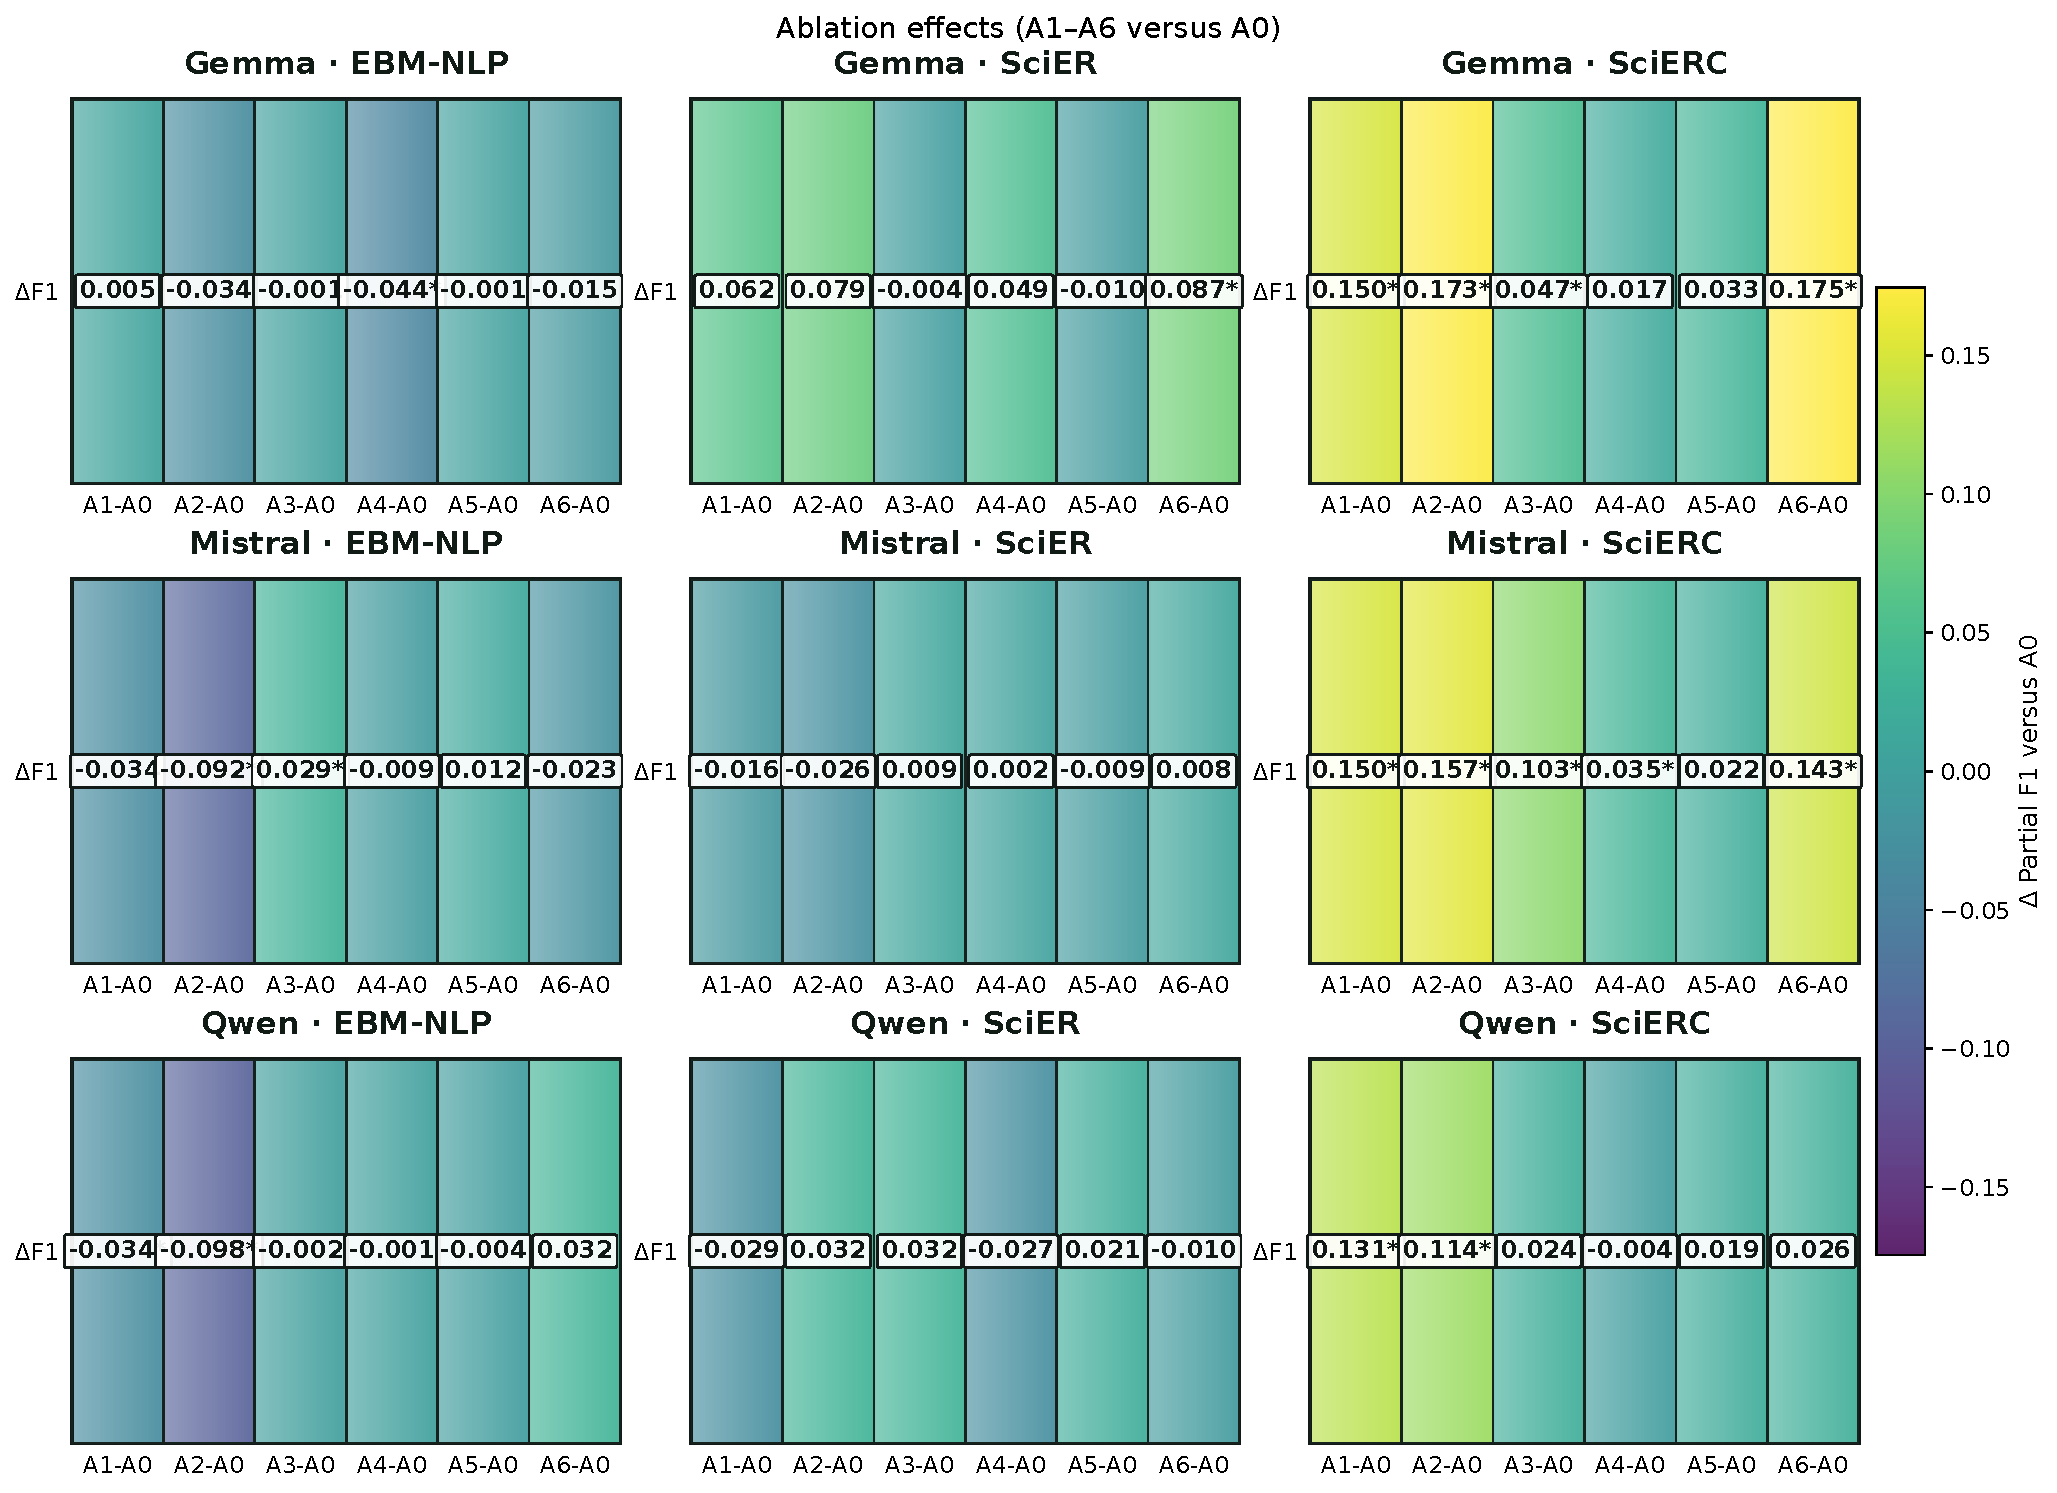
\includegraphics[width=\textwidth]{figs/appendix_visuals/r1_ablations_full.pdf}
    \caption{Visual summary of document-paired ablation effects. Each cell shows $\Delta$ partial F1 for A1--A6 relative to A0; asterisk marks Holm-adjusted $p<0.05$ within the corresponding model--dataset family.}
    \label{tab:r1-ablations-full}
\end{figure*}

\endgroup

\begingroup
\footnotesize
\setlength{\tabcolsep}{4pt}
\setlength{\LTleft}{0pt}
\setlength{\LTright}{0pt}
\begin{figure*}[t]
    \centering
    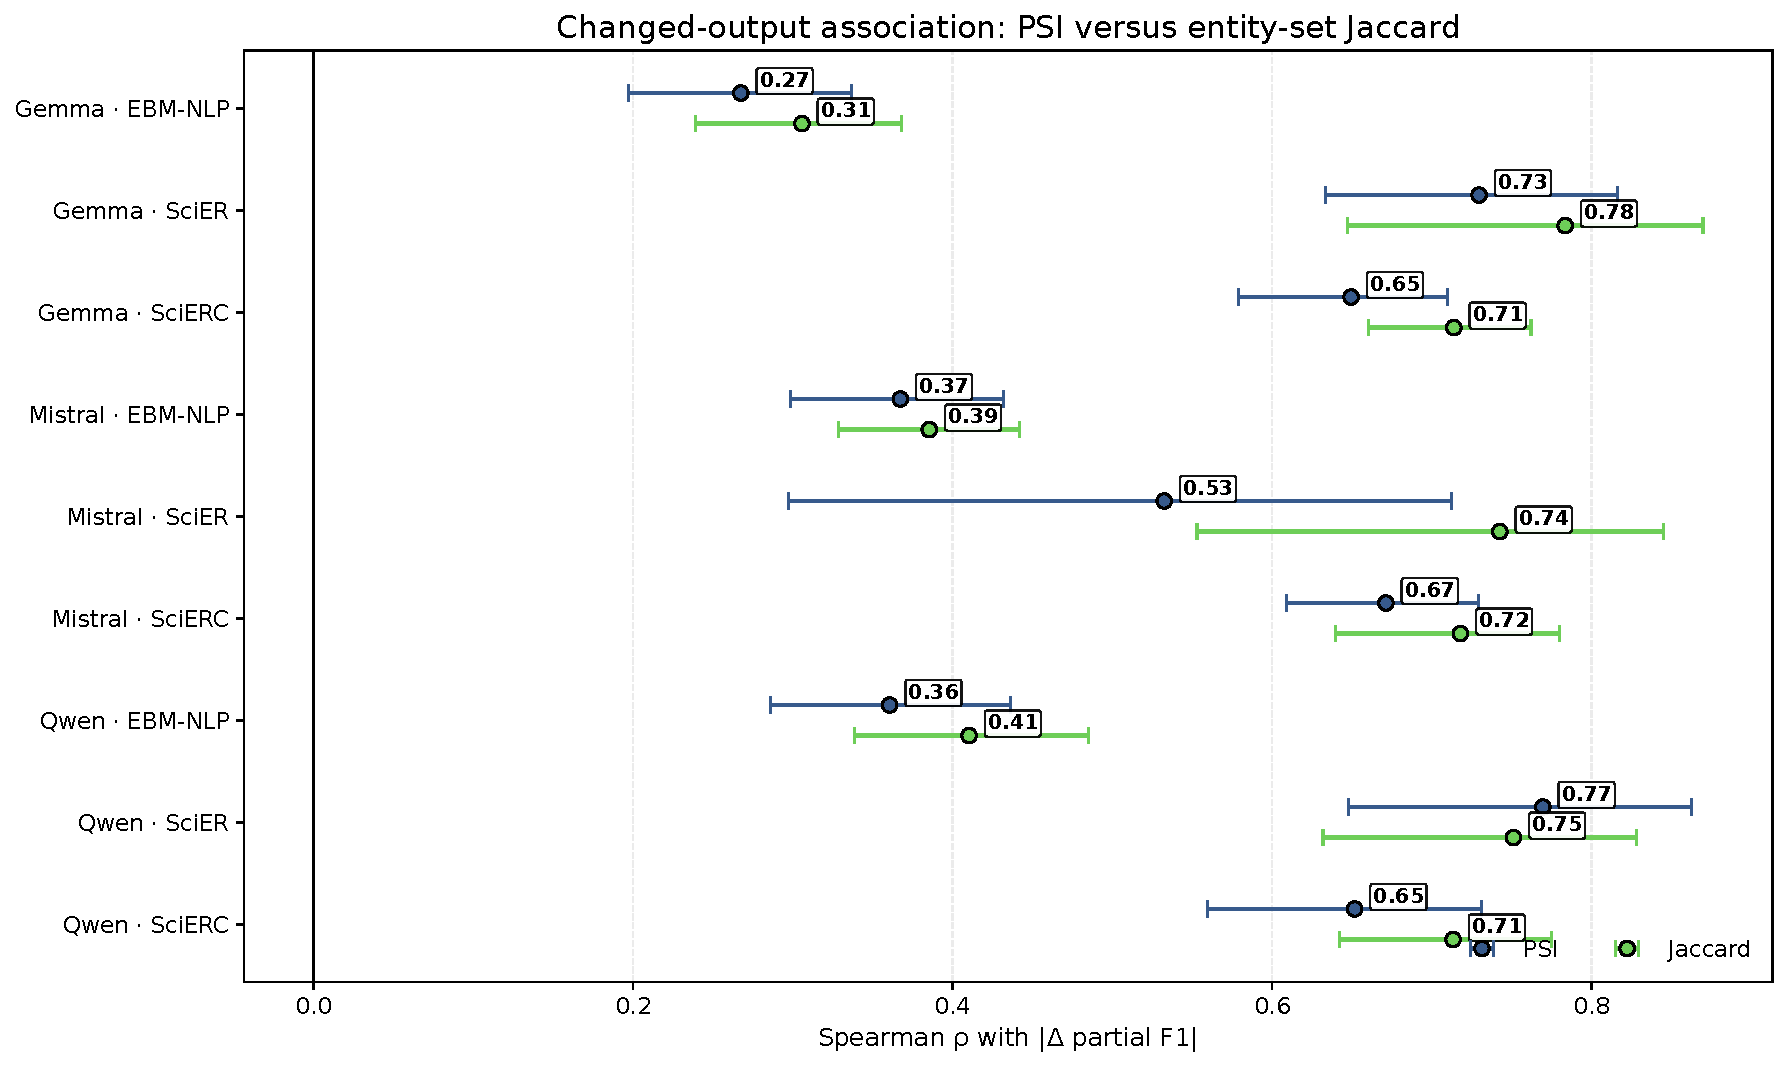
\includegraphics[width=\textwidth]{figs/appendix_visuals/r1_psi_jaccard_full.pdf}
    \caption{Changed-output transitions only: associations between output-change measures and absolute changes in partial entity F1. Points show Spearman $\rho$ with document-cluster bootstrap confidence intervals.}
    \label{tab:r1-psi-jaccard-full}
\end{figure*}

\endgroup

\begingroup
\footnotesize
\setlength{\tabcolsep}{4pt}
\setlength{\LTleft}{0pt}
\setlength{\LTright}{0pt}
\begin{figure*}[t]
    \centering
    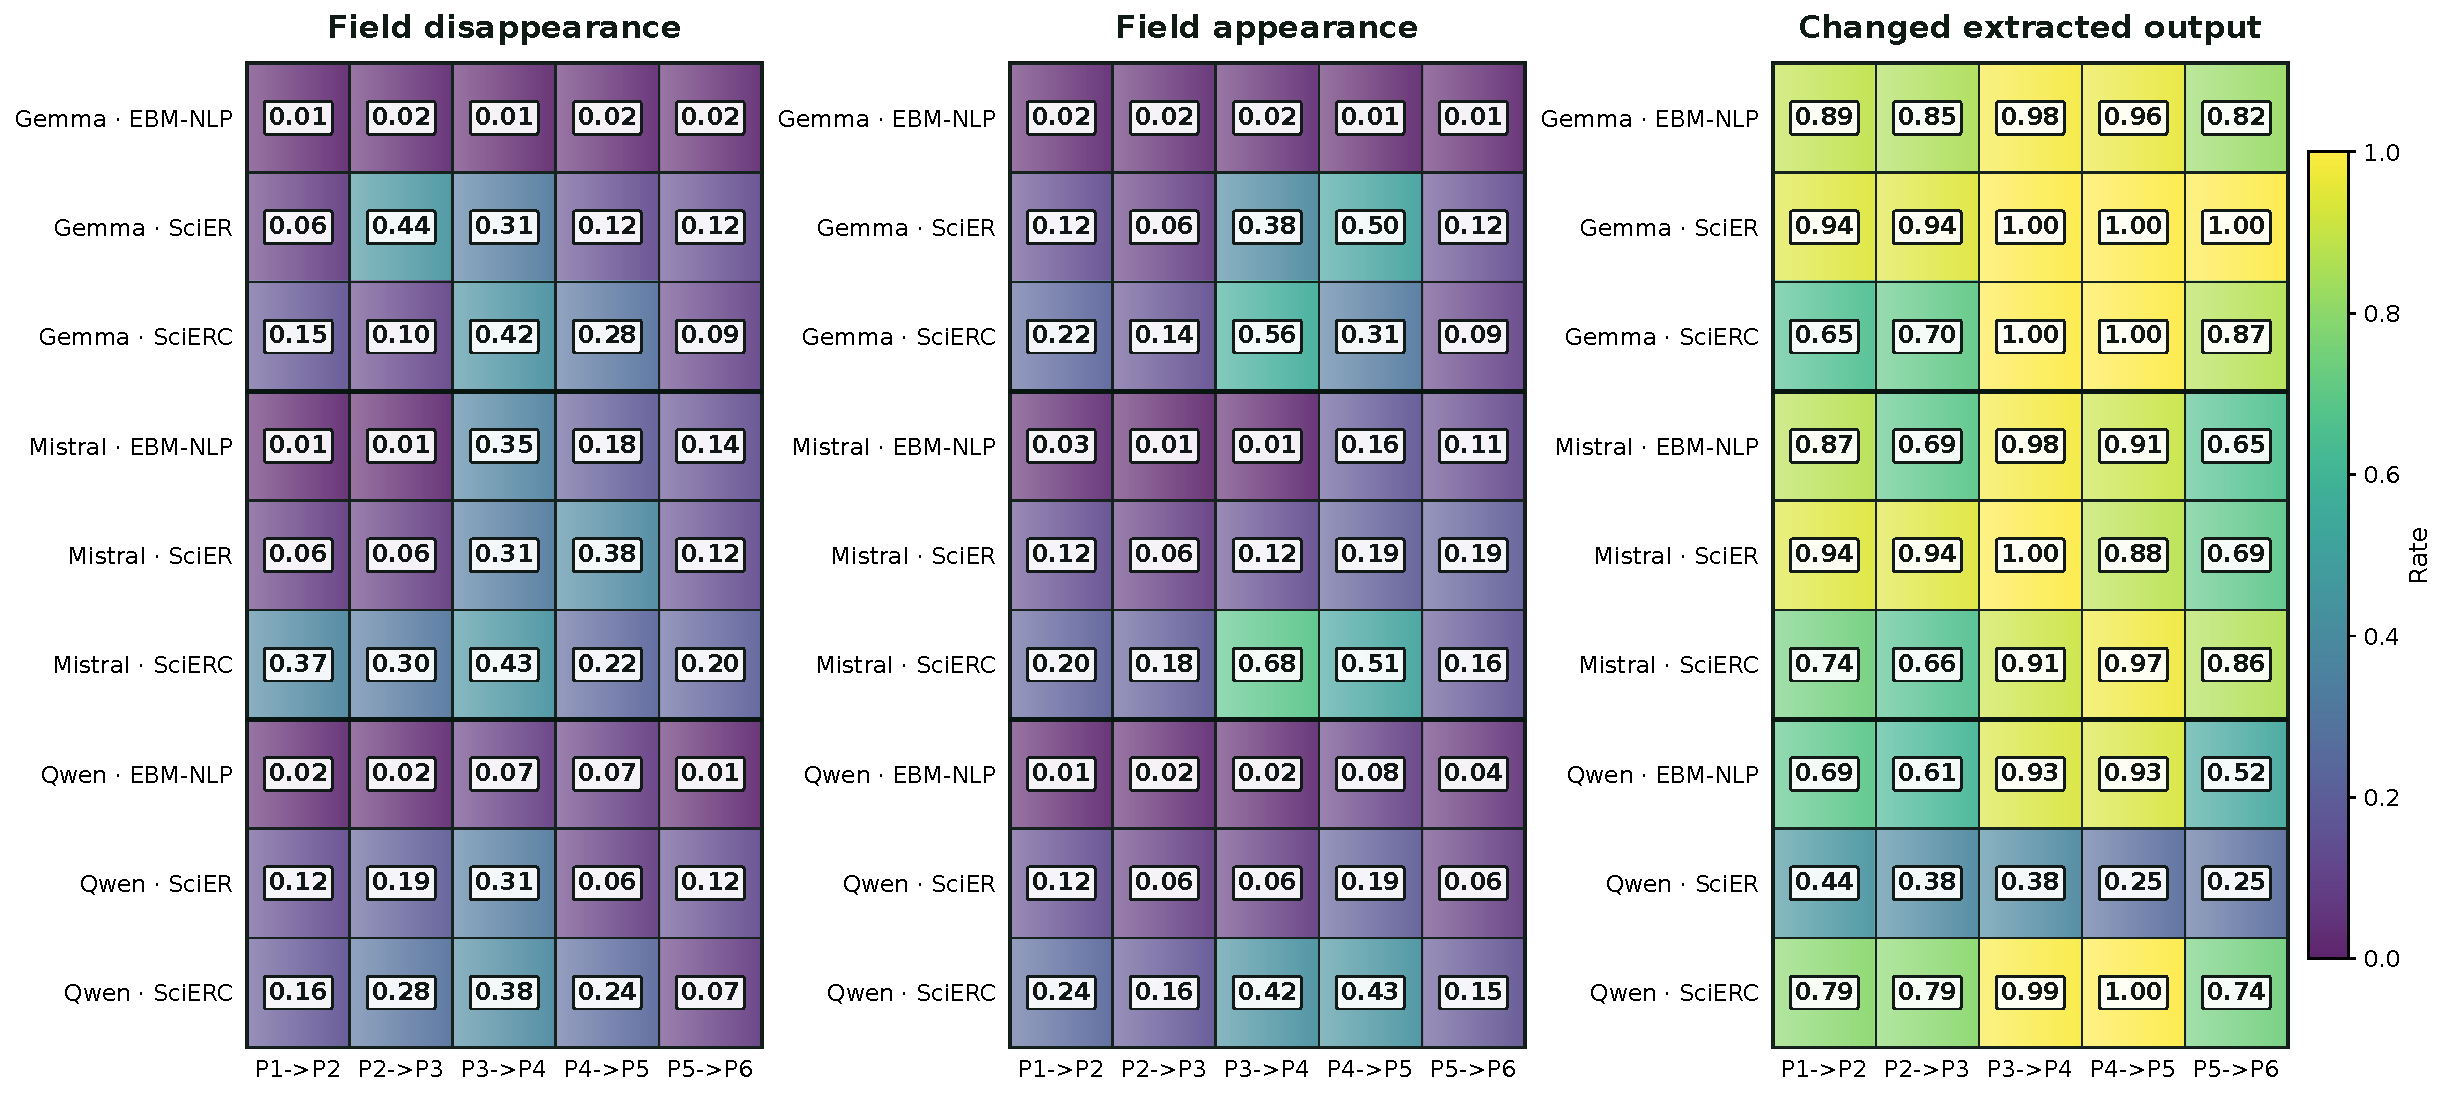
\includegraphics[width=\textwidth]{figs/appendix_visuals/r1_idr_full.pdf}
    \caption{Directional field disappearance, field appearance, and changed-output rates for each adjacent prompt transition, shown for all model--dataset cells.}
    \label{tab:r1-idr-full}
\end{figure*}

\endgroup

\begingroup
\footnotesize
\setlength{\tabcolsep}{4pt}
\setlength{\LTleft}{0pt}
\setlength{\LTright}{0pt}
\begin{figure*}[t]
    \centering
    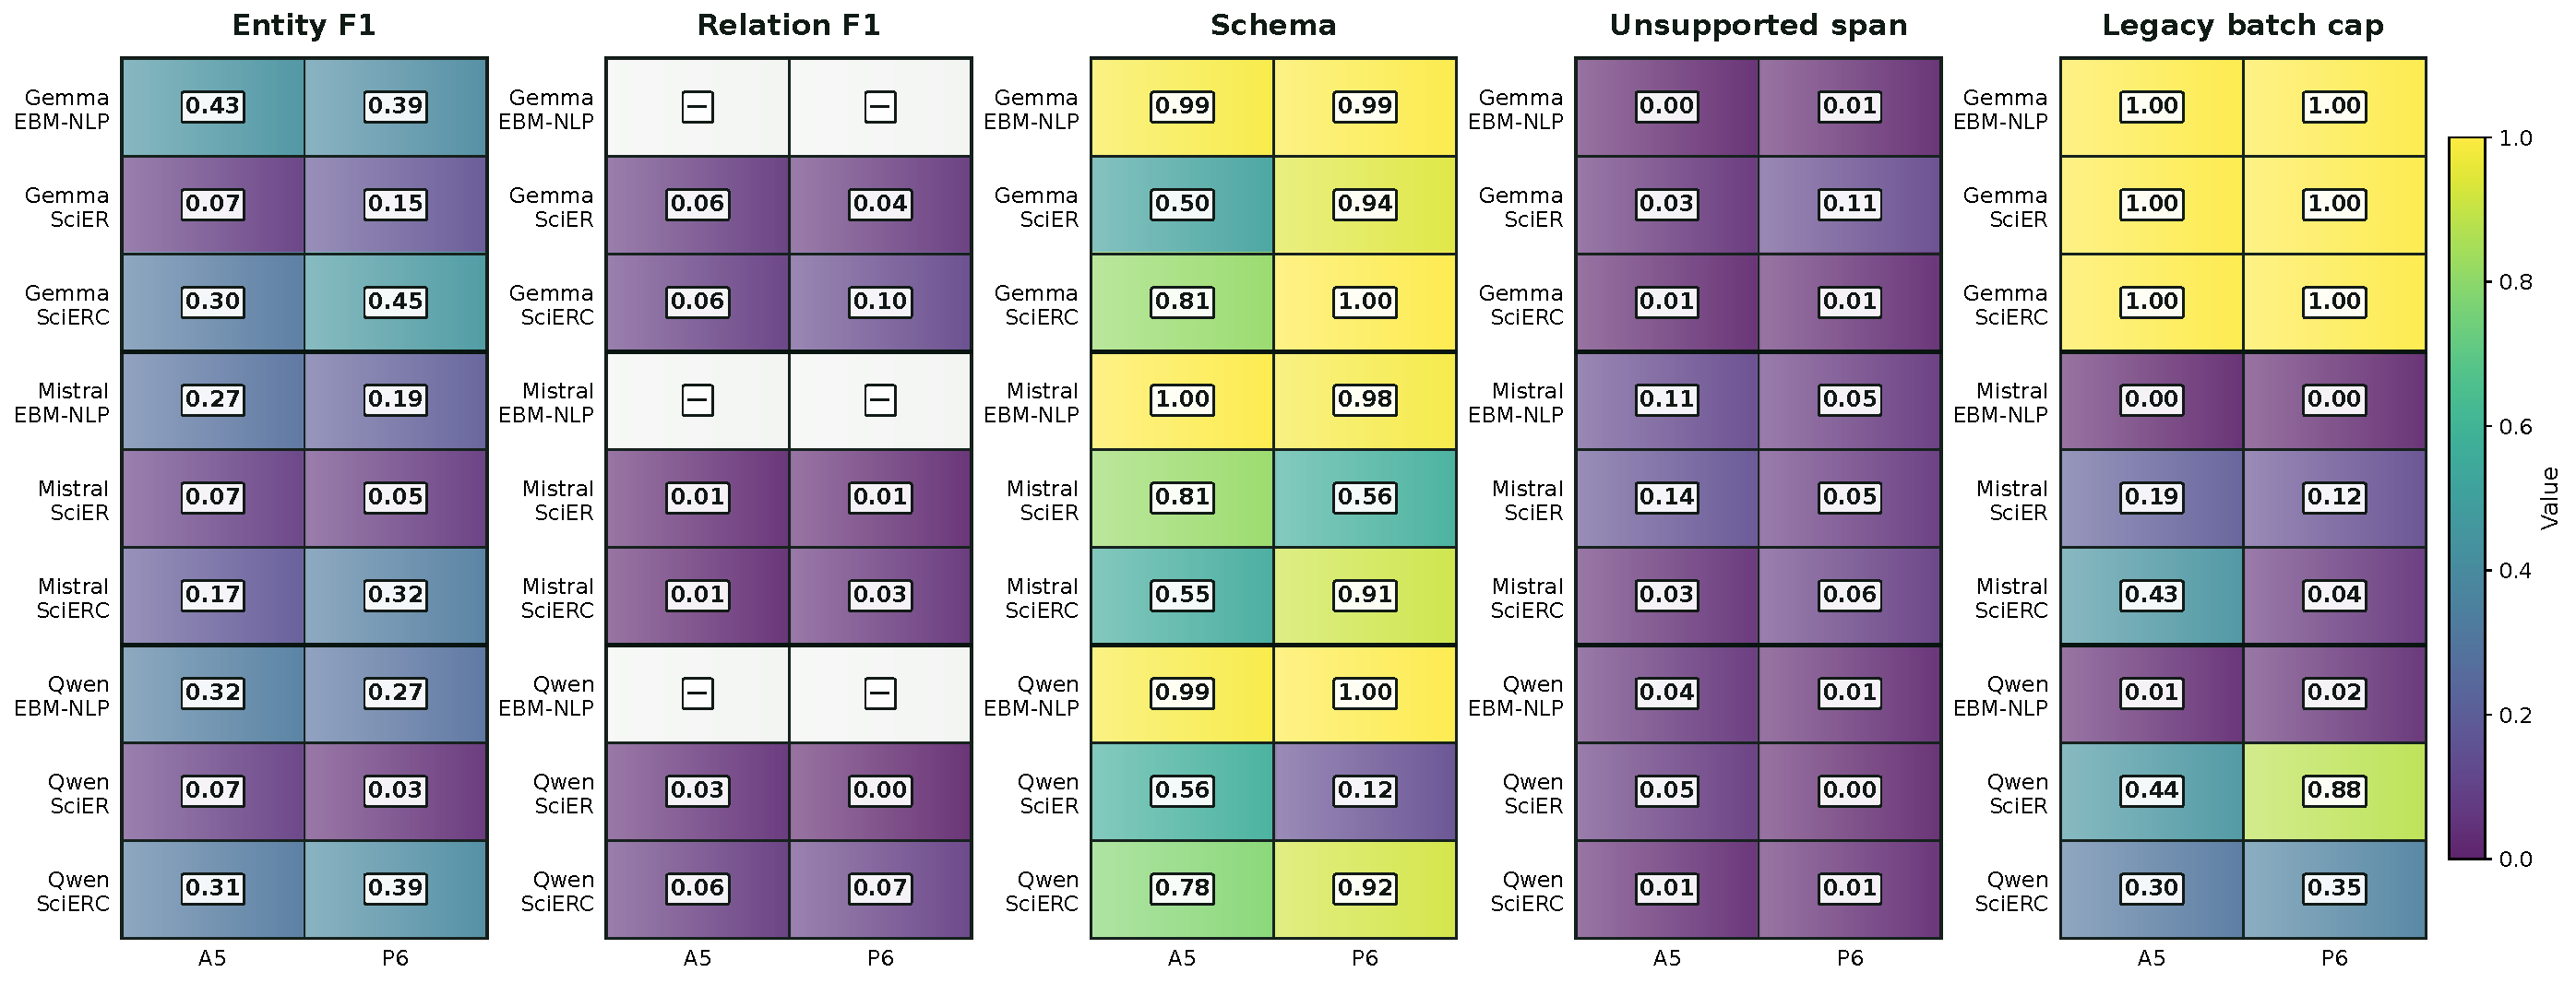
\includegraphics[width=\textwidth]{figs/appendix_visuals/r1_condition_quality.pdf}
    \caption{Observed A5/P6 condition-level quality and validity. Rows correspond to model--dataset cells; columns compare A5 and P6 for entity F1, relation F1, schema validity, unsupported-span rate, and the legacy batch-cap flag.}
    \label{tab:r1-condition-quality}
\end{figure*}

\endgroup

\begingroup
\footnotesize
\setlength{\tabcolsep}{4pt}
\setlength{\LTleft}{0pt}
\setlength{\LTright}{0pt}
\begin{figure*}[t]
    \centering
    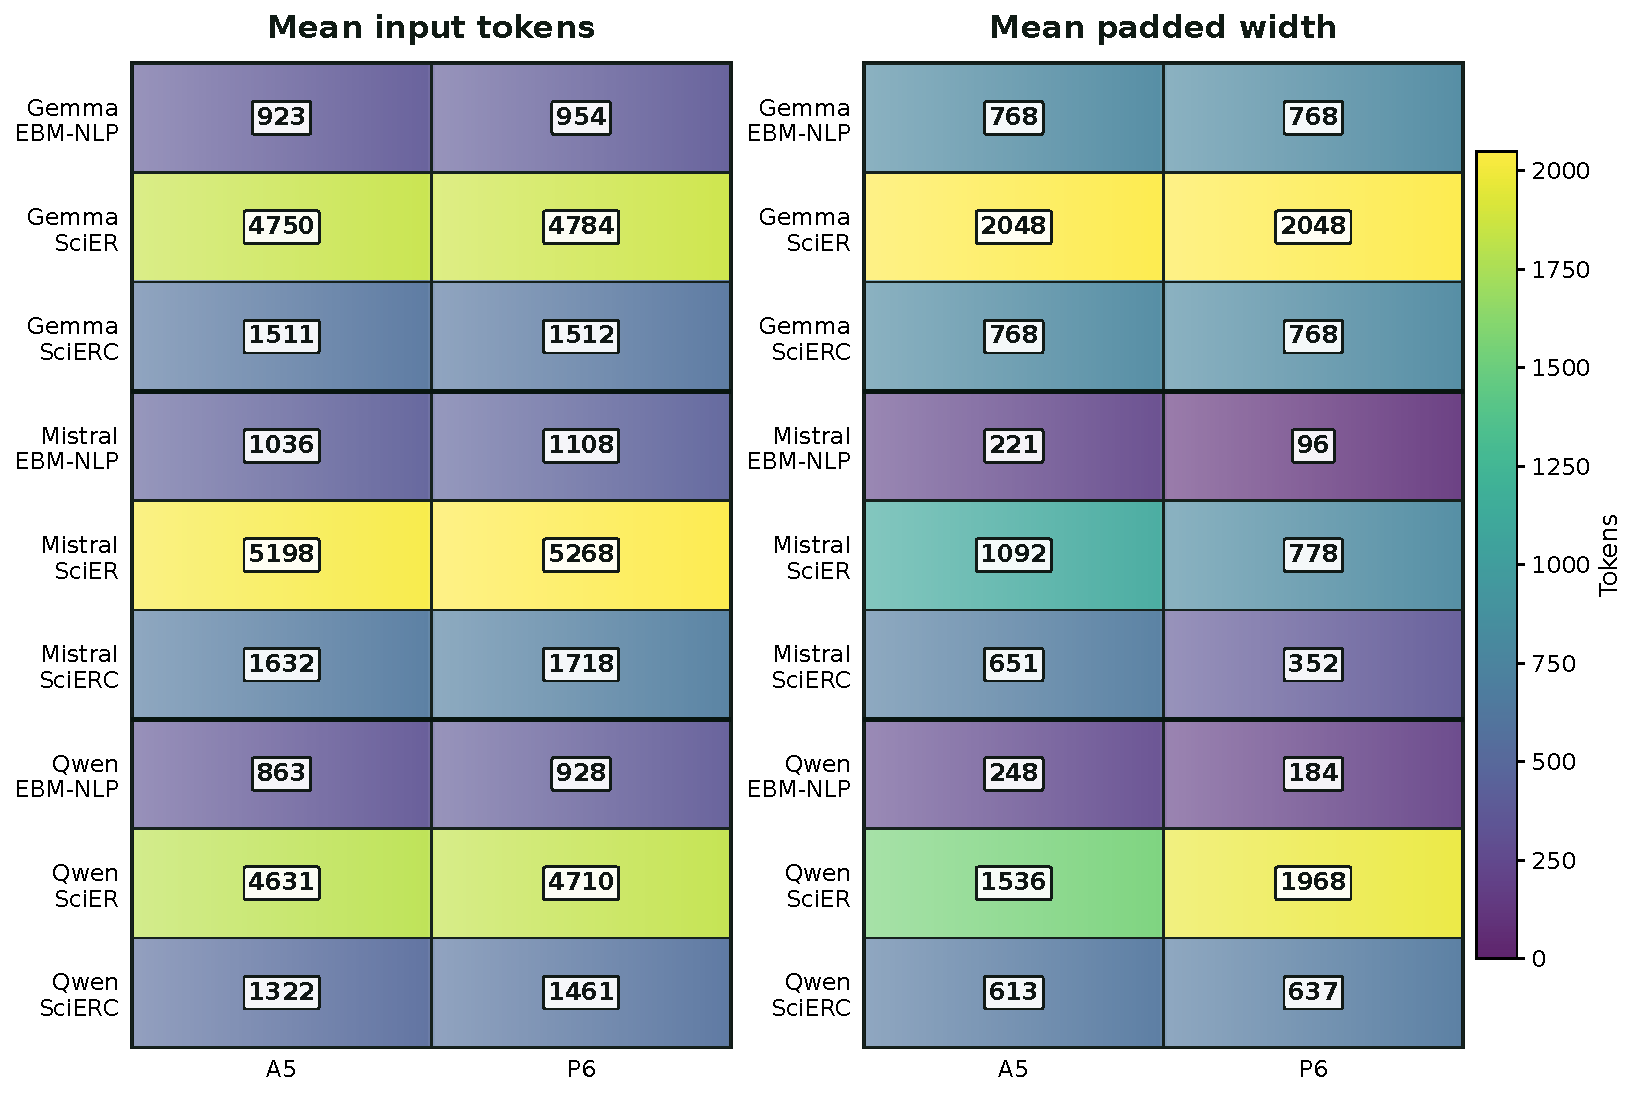
\includegraphics[width=\textwidth]{figs/appendix_visuals/r1_condition_tokens.pdf}
    \caption{Observed A5/P6 token budgets measured with each model tokenizer. Panels compare mean input-token counts and mean padded widths over the matched evaluation subsets.}
    \label{tab:r1-condition-tokens}
\end{figure*}

\endgroup

\begingroup
\footnotesize
\setlength{\tabcolsep}{4pt}
\setlength{\LTleft}{0pt}
\setlength{\LTright}{0pt}
\begin{figure*}[t]
    \centering
    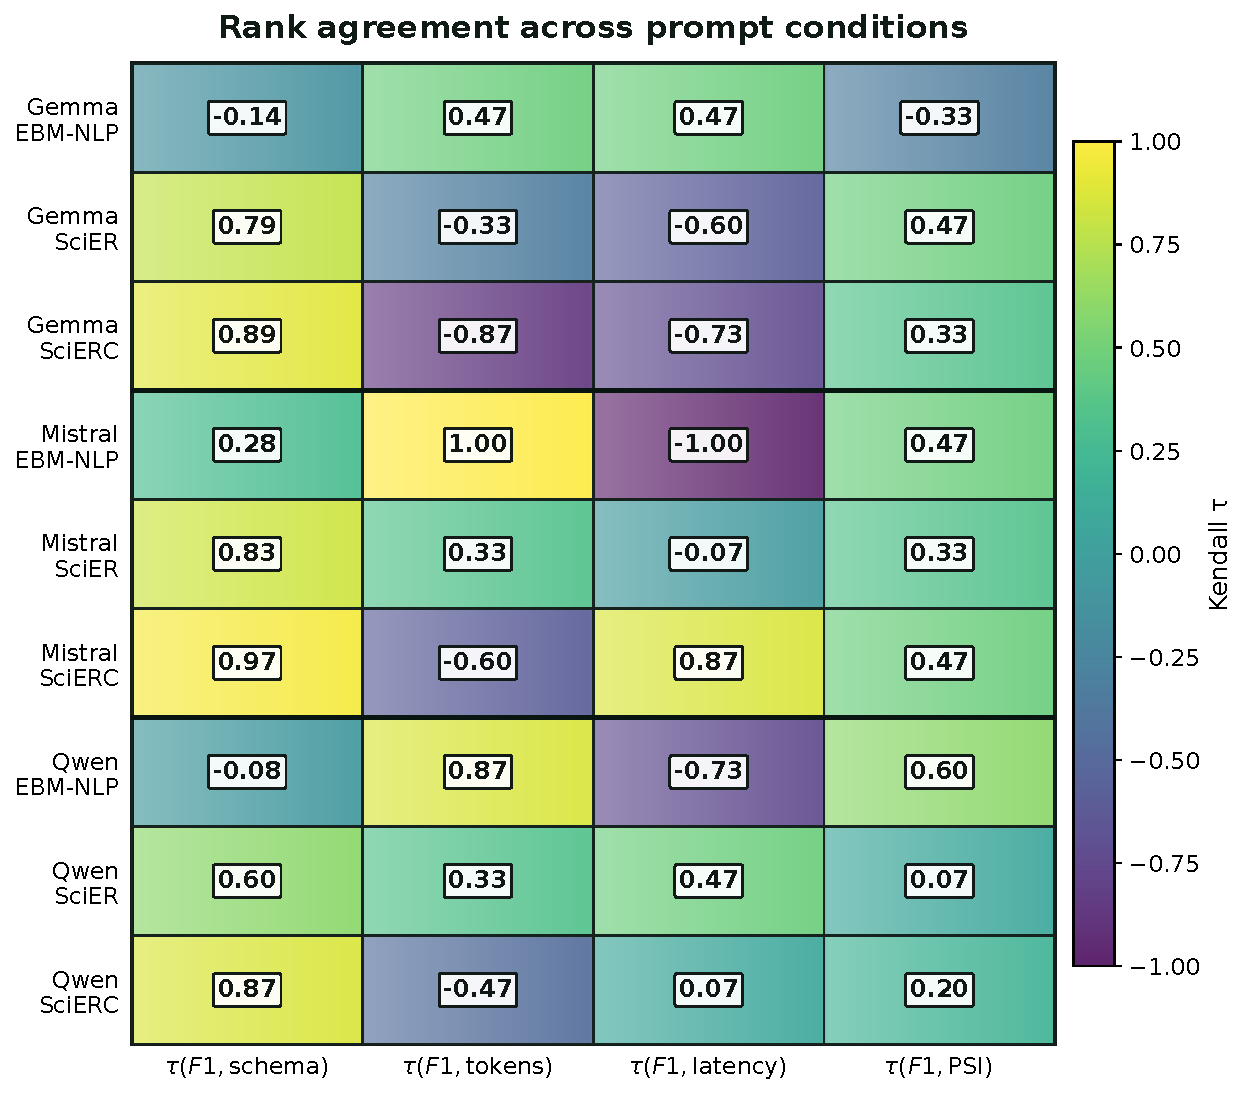
\includegraphics[width=\textwidth]{figs/appendix_visuals/r1_rq5_rank.pdf}
    \caption{Kendall rank agreement between extraction quality and competing criteria across the six prompt configurations. Positive values denote better directional agreement.}
    \label{tab:r1-rq5-rank}
\end{figure*}

\endgroup

\section{Unresolved validation analyses and interpretation boundaries}
\label{app:audit}
The existing published aggregate table supports token budgets, reference F1,
relation F1, schema validity, source-grounded hallucination, output-limit-hit
rates, and latency for all model--dataset--condition combinations. %% revised - reviewer #1 - comments 3-7 - Distinguish completed record-level analysis from experiments that remain genuinely unresolved.
The 9,726 evaluation records and 4,605 matched Phase~II transitions were
reprocessed using the paired analysis script. The resulting condition-level
metrics, Wilcoxon/Holm and rank-biserial estimates, McNemar comparisons,
PSI/Jaccard cluster intervals, Phase~II IDR and criterion-rank agreements are
reported in Appendix~\ref{app:posthoc-results}, with the matched P6--A5 tests
also shown in Table~\ref{tab:p6-a5-paired-all}.
%% revised - reviewer #1 - comments 1,2,8,11 - Historical experiment restored.
All 3,180 original Phase~I predictions and the executable P6 constructor
are recovered. Tables and figures in Phase~I Results are consistently
recalculated from the archived records. The historical log has no repeated
identical document--condition calls, so its 2025 run-to-run noise floor is
not identifiable. Prospective repetitions can estimate only the current
endpoint's variability. Alternative demonstration sets and an independent
text-only encoder are not claimed as completed Phase~II controls.

\bibliography{sample}

%\section*{Acknowledgements}
%Devices were
%fabricated at the ???


\end{document}
